% **************************************************************************************************************
% A Classic Thesis Style
% An Homage to The Elements of Typographic Style
%
% Copyright (C) 2012 Andr\'e Miede http://www.miede.de
%
% If you like the style then I would appreciate a postcard. My address 
% can be found in the file ClassicThesis.pdf. A collection of the 
% postcards I received so far is available online at 
% http://postcards.miede.de
%
% License:
% This program is free software; you can redistribute it and/or modify
% it under the terms of the GNU General Public License as published by
% the Free Software Foundation; either version 2 of the License, or
% (at your option) any later version.
%
% This program is distributed in the hope that it will be useful,
% but WITHOUT ANY WARRANTY; without even the implied warranty of
% MERCHANTABILITY or FITNESS FOR A PARTICULAR PURPOSE.  See the
% GNU General Public License for more details.
%
% You should have received a copy of the GNU General Public License
% along with this program; see the file COPYING.  If not, write to
% the Free Software Foundation, Inc., 59 Temple Place - Suite 330,
% Boston, MA 02111-1307, USA.
%
% **************************************************************************************************************
% Note:
%    * You must not use "u etc. in strings/commands that will be spaced out (use \"u or real umlauts instead)
%    * New enumeration (small caps): \begin{aenumerate} \end{aenumerate}
%    * For margin notes: \marginpar or \graffito{}
%    * Do not use bold fonts in this style, it is designed around them
%    * Use tables as in the examples
%    * See classicthesis-preamble.sty for useful commands
% **************************************************************************************************************
% To Do:
%		 * [high] Check this out: http://www.golatex.de/koma-script-warnung-in-verbindung-mit-listings-package-t2058.html
%    * [medium] mathbb in section-titles/chapter-titles => disappears somehow in headlines!!!
% **************************************************************************************************************
\documentclass[ twoside,openright,titlepage,numbers=noenddot,headinclude,%1headlines,% letterpaper a4paper
                footinclude=true,cleardoublepage=empty,abstractoff, % <--- obsolete, remove (todo)
                BCOR=5mm,paper=a4,fontsize=11pt,%11pt,a4paper,%
                ngerman,american,%
                ]{scrreprt}

%********************************************************************
% Note: Make all your adjustments in here
%*******************************************************
% ****************************************************************************************************
% classicthesis-config.tex 
% formerly known as loadpackages.sty, classicthesis-ldpkg.sty, and classicthesis-preamble.sty 
% Use it at the beginning of your ClassicThesis.tex, or as a LaTeX Preamble 
% in your ClassicThesis.{tex,lyx} with % ****************************************************************************************************
% classicthesis-config.tex 
% formerly known as loadpackages.sty, classicthesis-ldpkg.sty, and classicthesis-preamble.sty 
% Use it at the beginning of your ClassicThesis.tex, or as a LaTeX Preamble 
% in your ClassicThesis.{tex,lyx} with % ****************************************************************************************************
% classicthesis-config.tex 
% formerly known as loadpackages.sty, classicthesis-ldpkg.sty, and classicthesis-preamble.sty 
% Use it at the beginning of your ClassicThesis.tex, or as a LaTeX Preamble 
% in your ClassicThesis.{tex,lyx} with \input{classicthesis-config}
% ****************************************************************************************************  
% If you like the classicthesis, then I would appreciate a postcard. 
% My address can be found in the file ClassicThesis.pdf. A collection 
% of the postcards I received so far is available online at 
% http://postcards.miede.de
% ****************************************************************************************************

% ****************************************************************************************************
% 1. Configure classicthesis for your needs here, e.g., remove "drafting" below 
% in order to deactivate the time-stamp on the pages
% ****************************************************************************************************
\PassOptionsToPackage{eulerchapternumbers,listings,drafting,%
				 pdfspacing,%floatperchapter,%linedheaders,%
				 subfig,beramono,eulermath,parts}{classicthesis}										
% ********************************************************************
% Available options for classicthesis.sty 
% (see ClassicThesis.pdf for more information):
% drafting
% parts nochapters linedheaders
% eulerchapternumbers beramono eulermath pdfspacing minionprospacing
% tocaligned dottedtoc manychapters
% listings floatperchapter subfig
% ********************************************************************

% ********************************************************************
% Triggers for this config
% ******************************************************************** 
\usepackage{ifthen}
\newboolean{enable-backrefs} % enable backrefs in the bibliography
\setboolean{enable-backrefs}{true} % true false
% ****************************************************************************************************


% ****************************************************************************************************
% 2. Personal data and user ad-hoc commands
% ****************************************************************************************************
\newcommand{\myTitle}{Combining Linked Data and Statistical Information Retrieval - Next Generation Search Engine}
%\newcommand{\mySubtitle}{An Homage to The Elements of Typographic Style\xspace}
\newcommand{\myDegree}{Dissertation\xspace}
\newcommand{\myName}{Ricardo Usbeck\xspace}
\newcommand{\myProf}{Prof. Dr. Ing. habil. Klaus-Peter Fa\"hnrich\xspace}
\newcommand{\myOtherProf}{Put name here\xspace}
\newcommand{\mySupervisor}{Dr. Axel-Cyrille Ngonga Ngomo\xspace}
\newcommand{\myFaculty}{Fakult\"at f\"ur Mathematik und Informatik\xspace}
\newcommand{\myDepartment}{Abteilung f\"ur Betriebliche Informationssysteme\xspace}
\newcommand{\myUni}{Universit\"at Leipzig\xspace}
\newcommand{\myLocation}{Universit\"at Leipzig\xspace}
\newcommand{\myTime}{January 2013 - September 2015\xspace}
%\newcommand{\myVersion}{version 4.1\xspace}

% ********************************************************************
% Setup, finetuning, and useful commands
% ********************************************************************
\newcounter{dummy} % necessary for correct hyperlinks (to index, bib, etc.)
\newlength{\abcd} % for ab..z string length calculation
\providecommand{\mLyX}{L\kern-.1667em\lower.25em\hbox{Y}\kern-.125emX\@}
\newcommand{\ie}{i.\,e.}
\newcommand{\Ie}{I.\,e.}
\newcommand{\eg}{e.\,g.}
\newcommand{\Eg}{E.\,g.} 
% ****************************************************************************************************


% ****************************************************************************************************
% 3. Loading some handy packages
% ****************************************************************************************************
% ******************************************************************** 
% Packages with options that might require adjustments
% ******************************************************************** 
%\PassOptionsToPackage{latin9}{inputenc}	% latin9 (ISO-8859-9) = latin1+"Euro sign"
% \usepackage{inputenc}				
\usepackage[T1]{fontenc}

%\PassOptionsToPackage{ngerman,american}{babel}   % change this to your language(s)
% Spanish languages need extra options in order to work with this template
%\PassOptionsToPackage{spanish,es-lcroman}{babel}
 \usepackage{babel}					

%\PassOptionsToPackage{square,numbers}{natbib}
% \usepackage{natbib}		
\hyphenation{Leh-mann}
 \usepackage[authoryear,square,colon]{natbib}		
 
%\PassOptionsToPackage{fleqn}{amsmath}		% math environments and more by the AMS 
% \usepackage{amsmath}


% ******************************************************************** 
% General useful packages
% ******************************************************************** 
\PassOptionsToPackage{T1}{fontenc} % T2A for cyrillics
	\usepackage{fontenc}     
\usepackage{textcomp} % fix warning with missing font shapes
\usepackage{scrhack} % fix warnings when using KOMA with listings package          
\usepackage{xspace} % to get the spacing after macros right  
\usepackage{mparhack} % get marginpar right
\usepackage{fixltx2e} % fixes some LaTeX stuff 
\PassOptionsToPackage{printonlyused,smaller}{acronym}
	\usepackage{acronym} % nice macros for handling all acronyms in the thesis
%\renewcommand*{\acsfont}[1]{\textssc{#1}} % for MinionPro
%\renewcommand{\bflabel}[1]{{#1}\hfill} % fix the list of acronyms
% ****************************************************************************************************


% ****************************************************************************************************
% 4. Setup floats: tables, (sub)figures, and captions
% ****************************************************************************************************
\usepackage{tabularx} % better tables
	\setlength{\extrarowheight}{3pt} % increase table row height
\newcommand{\tableheadline}[1]{\multicolumn{1}{c}{\spacedlowsmallcaps{#1}}}
\newcommand{\myfloatalign}{\centering} % to be used with each float for alignment
\usepackage{caption}
\captionsetup{format=hang,font=small}
\usepackage{subfig}  
% ****************************************************************************************************


% ****************************************************************************************************    		   


% ****************************************************************************************************
% 6. PDFLaTeX, hyperreferences and citation backreferences
% ****************************************************************************************************
% ********************************************************************
% Using PDFLaTeX
% ********************************************************************
\PassOptionsToPackage{pdftex,hyperfootnotes=false,pdfpagelabels,breaklinks}{hyperref}
	\usepackage{hyperref}  % backref linktocpage pagebackref
\pdfcompresslevel=9
\pdfadjustspacing=1 
\PassOptionsToPackage{pdftex}{graphicx}
	\usepackage{graphicx} 
\usepackage{wrapfig}
% ********************************************************************
% Setup the style of the backrefs from the bibliography
% (translate the options to any language you use)
% ********************************************************************
\newcommand{\backrefnotcitedstring}{\relax}%(Not cited.)
\newcommand{\backrefcitedsinglestring}[1]{(Cited on page~#1.)}
\newcommand{\backrefcitedmultistring}[1]{(Cited on pages~#1.)}
\ifthenelse{\boolean{enable-backrefs}}%
{%
		\PassOptionsToPackage{hyperpageref}{backref}
		\usepackage{backref} % to be loaded after hyperref package 
		   \renewcommand{\backreftwosep}{ and~} % separate 2 pages
		   \renewcommand{\backreflastsep}{, and~} % separate last of longer list
		   \renewcommand*{\backref}[1]{}  % disable standard
		   \renewcommand*{\backrefalt}[4]{% detailed backref
		      \ifcase #1 %
		         \backrefnotcitedstring%
		      \or%
		         \backrefcitedsinglestring{#2}%
		      \else%
		         \backrefcitedmultistring{#2}%
		      \fi}%
}{\relax}    

% ********************************************************************
% Hyperreferences
% ********************************************************************
\hypersetup{%
    %draft,	% = no hyperlinking at all (useful in b/w printouts)
    colorlinks=true, linktocpage=true, pdfstartpage=3, pdfstartview=FitV,%
    % uncomment the following line if you want to have black links (e.g., for printing)
    %colorlinks=false, linktocpage=false, pdfborder={0 0 0}, pdfstartpage=3, pdfstartview=FitV,% 
    breaklinks=true, pdfpagemode=UseNone, pageanchor=true, pdfpagemode=UseOutlines,%
    plainpages=false, bookmarksnumbered, bookmarksopen=true, bookmarksopenlevel=1,%
    hypertexnames=true, pdfhighlight=/O,%nesting=true,%frenchlinks,%
    urlcolor=webbrown, linkcolor=RoyalBlue, citecolor=webgreen, %pagecolor=RoyalBlue,%
    %urlcolor=Black, linkcolor=Black, citecolor=Black, %pagecolor=Black,%
    pdftitle={\myTitle},%
    pdfauthor={\textcopyright\ \myName, \myUni, \myFaculty},%
    pdfsubject={},%
    pdfkeywords={},%
    pdfcreator={pdfLaTeX},%
    pdfproducer={LaTeX with hyperref and classicthesis}%
}   

% ********************************************************************
% Setup autoreferences
% ********************************************************************
% There are some issues regarding autorefnames
% http://www.ureader.de/msg/136221647.aspx
% http://www.tex.ac.uk/cgi-bin/texfaq2html?label=latexwords
% you have to redefine the makros for the 
% language you use, e.g., american, ngerman
% (as chosen when loading babel/AtBeginDocument)
% ********************************************************************
\makeatletter
\@ifpackageloaded{babel}%
    {%
       \addto\extrasamerican{%
					\renewcommand*{\figureautorefname}{Figure}%
					\renewcommand*{\tableautorefname}{Table}%
					\renewcommand*{\partautorefname}{Part}%
					\renewcommand*{\chapterautorefname}{Chapter}%
					\renewcommand*{\sectionautorefname}{Section}%
					\renewcommand*{\subsectionautorefname}{Section}%
					\renewcommand*{\subsubsectionautorefname}{Section}% 	
				}%
       \addto\extrasngerman{% 
					\renewcommand*{\paragraphautorefname}{Absatz}%
					\renewcommand*{\subparagraphautorefname}{Unterabsatz}%
					\renewcommand*{\footnoteautorefname}{Fu\"snote}%
					\renewcommand*{\FancyVerbLineautorefname}{Zeile}%
					\renewcommand*{\theoremautorefname}{Theorem}%
					\renewcommand*{\appendixautorefname}{Anhang}%
					\renewcommand*{\equationautorefname}{Gleichung}%        
					\renewcommand*{\itemautorefname}{Punkt}%
				}%	
			% Fix to getting autorefs for subfigures right (thanks to Belinda Vogt for changing the definition)
			\providecommand{\subfigureautorefname}{\figureautorefname}%  			
    }{\relax}
\makeatother


% ****************************************************************************************************
% 7. Last calls before the bar closes
% ****************************************************************************************************
% ********************************************************************
% Development Stuff
% ********************************************************************
\listfiles
%\PassOptionsToPackage{l2tabu,orthodox,abort}{nag}
%	\usepackage{nag}
%\PassOptionsToPackage{warning, all}{onlyamsmath}
%	\usepackage{onlyamsmath}

% ********************************************************************
% Last, but not least...
% ********************************************************************
\usepackage{classicthesis} 
% ****************************************************************************************************

% ****************************************************************************************************
% 5. Setup code listings
% ****************************************************************************************************
\usepackage{listings} 
\lstset{
    numberbychapter=false,
    numbers=left,
    numberstyle=\tiny,
    basicstyle=\ttfamily\fontsize{8}{8}\selectfont,
    tabsize=2,
    framexleftmargin=2pt,
    captionpos=b,
    frame=single,
    breaklines=true,
    aboveskip=1.5em
}

\lstset{literate=%
{Ö}{{\"O}}1
{Ä}{{\"A}}1
{Ü}{{\"U}}1
{ß}{{\ss}}2
{ü}{{\"u}}1
{ä}{{\"a}}1
{ö}{{\"o}}1
{é}{{\'e}}1
}

% Turtle box
%\usepackage{color}
%\usepackage{xcolor}
\definecolor{olivegreen}{rgb}{0.1,0.6,0.3}
\definecolor{grey}{rgb}{0.2,0.2,0.2}
\lstdefinelanguage{ttl}{
sensitive=true,
showstringspaces=false,
morecomment=[l][\color{cyan}]{@prefix},
morecomment=[l][\color{webbrown}]{@de},
morecomment=[l][\color{webbrown}]{@en},
morecomment=[l][\color{webbrown}]{@fr},
morecomment=[l][\color{olivegreen}]{\#},
morestring=[b][\color{olivegreen}]\",
keywordstyle=\color{cyan},
morekeywords={version,owl,rdf,rdfs,xml,xsd,dbo,str,sso,scms,ld, fise, dcterms, itsrdf, wiktionary, nif, rlno, dbpedia,rlnr, frdbr, dedbr, skos, dbr, prefix, fbase, rdfs, dbo}
}

%\lstdefinestyle{rdf}{numberblanklines=true, morekeywords={}}
%\lstdefinestyle{sparql}{numberblanklines=true, morekeywords={SELECT,WHERE FILTER, GROUP BY, IN, AS}}
\lstdefinestyle{N3}{numberblanklines=true, morekeywords={foaf, prefix}}

\usepackage{lipsum}
\usepackage{todonotes}
\usepackage{paralist}
\usepackage{amsmath}%, amsthm, amssymb, array}
\usepackage{amssymb}


%%%%%%%%%%%%%%%%%%%%%%%%% START TBSL %%%%%%%%%%%%%%%%%%%%%%%%%

\usepackage{enumitem}
%\usepackage[usenames,dvipsnames]{color}
%\usepackage[table]{xcolor}
\newcommand{\sparqlwo}[2]{{\texttt{#1 \char '173} \\[1.5pt] \hspace*{.5cm}\parbox{6cm}{\tt #2} \\ \texttt{\char '175} }}
\newcommand{\sparql}[3]{{\texttt{#1 \char '173} \\[1.5pt] \hspace*{.5cm}\parbox{6cm}{\tt #2} \\ \texttt{\char '175} \\ \texttt{#3} }}
\newcommand{\slot}[3]{$\langle\texttt{#1},\text{#2},\text{\sf #3}\rangle$}
\newcommand{\argmax}{\operatornamewithlimits{arg\,max}}
\newcommand{\argmin}{\operatornamewithlimits{arg\,min}}

\usepackage{qtree}

\newcommand{\Drs}[2]{%%%%%%%%%%%%%%%%%%%%%%%%%
\(                   % begin maths mode
 \begin{array}{|l|}  %
 \hline              % top line
   \begin{array}{l}  %
    #1                % `Universe'
    \end{array} \\   %  end the `universe' part
 \hline              % line between Universe and Conditions
    \begin{array}{l} %
    #2                % the conditions
    \end{array} \\   % end the conditions part
 \hline              % bottom line
\end{array}          %
\)                   % end maths mode
                     }%%%%%%%%%%%%%%%%%%%%%%%%%
                     
%%%%%%%%%%%%%%%%%%%%%%%%% END TBSL %%%%%%%%%%%%%%%%%%%%%%%%%                    

% landscape tables
% option 1
\usepackage{rotating}
\usepackage{longtable}
% option 2
\usepackage{lscape}
% force tables to be on a certain page, use H in \begin{table}[H]
%\usepackage{float}
%\restylefloat{table}

%\usepackage{refcheck}

\usepackage[utf8]{inputenc}
% fix the duplicate todo notes
\let\marginpar\oldmarginpar

%\newcommand{\Rdflivenews}{RdfLiveNews}
%\newcommand{\DEFACTO}{DeFacto}
%\newcommand{\FACTBENCH}{FactBench}
\newcommand{\Tau}{\mathfrak{T}}

\newtheorem{definition}{Definition}
% remove columns from tables
\newcolumntype{H}{>{\setbox0=\hbox\bgroup}c<{\egroup}@{}}

% insert häkchen für ja/nein tabellen
\usepackage{tikz}
\def\checkmark{\tikz\fill[scale=0.4](0,.35) -- (.25,0) -- (1,.7) -- (.25,.15) -- cycle;} 


\usepackage{pifont}% http://ctan.org/pkg/pifont
\newcommand{\cmark}{\ding{51}}%
\newcommand{\xmark}{\ding{55}}%

%\usepackage{tablefootnote}
\usepackage{afterpage}


% ****************************************************************************************************
% 8. Further adjustments (experimental)
% ****************************************************************************************************
% ********************************************************************
% Changing the text area
% ********************************************************************
\linespread{1} % a bit more for Palatino
\areaset[current]{400pt}{761pt} % 686 (factor 2.2) + 33 head + 42 head \the\footskip
%\setlength{\marginparwidth}{7em}%
%\setlength{\marginparsep}{2em}%

% ********************************************************************
% Using different fonts
% ********************************************************************
%\usepackage[oldstylenums]{kpfonts} % oldstyle notextcomp
%\usepackage[osf]{libertine}
%\usepackage{hfoldsty} % Computer Modern with osf
%\usepackage[light,condensed,math]{iwona}
%\renewcommand{\sfdefault}{iwona}
%\usepackage{lmodern} % <-- no osf support :-(
%\usepackage[urw-garamond]{mathdesign} <-- no osf support :-(
% ****************************************************************************************************

% ****************************************************************************************************  
% If you like the classicthesis, then I would appreciate a postcard. 
% My address can be found in the file ClassicThesis.pdf. A collection 
% of the postcards I received so far is available online at 
% http://postcards.miede.de
% ****************************************************************************************************

% ****************************************************************************************************
% 1. Configure classicthesis for your needs here, e.g., remove "drafting" below 
% in order to deactivate the time-stamp on the pages
% ****************************************************************************************************
\PassOptionsToPackage{eulerchapternumbers,listings,drafting,%
				 pdfspacing,%floatperchapter,%linedheaders,%
				 subfig,beramono,eulermath,parts}{classicthesis}										
% ********************************************************************
% Available options for classicthesis.sty 
% (see ClassicThesis.pdf for more information):
% drafting
% parts nochapters linedheaders
% eulerchapternumbers beramono eulermath pdfspacing minionprospacing
% tocaligned dottedtoc manychapters
% listings floatperchapter subfig
% ********************************************************************

% ********************************************************************
% Triggers for this config
% ******************************************************************** 
\usepackage{ifthen}
\newboolean{enable-backrefs} % enable backrefs in the bibliography
\setboolean{enable-backrefs}{true} % true false
% ****************************************************************************************************


% ****************************************************************************************************
% 2. Personal data and user ad-hoc commands
% ****************************************************************************************************
\newcommand{\myTitle}{Combining Linked Data and Statistical Information Retrieval - Next Generation Search Engine}
%\newcommand{\mySubtitle}{An Homage to The Elements of Typographic Style\xspace}
\newcommand{\myDegree}{Dissertation\xspace}
\newcommand{\myName}{Ricardo Usbeck\xspace}
\newcommand{\myProf}{Prof. Dr. Ing. habil. Klaus-Peter Fa\"hnrich\xspace}
\newcommand{\myOtherProf}{Put name here\xspace}
\newcommand{\mySupervisor}{Dr. Axel-Cyrille Ngonga Ngomo\xspace}
\newcommand{\myFaculty}{Fakult\"at f\"ur Mathematik und Informatik\xspace}
\newcommand{\myDepartment}{Abteilung f\"ur Betriebliche Informationssysteme\xspace}
\newcommand{\myUni}{Universit\"at Leipzig\xspace}
\newcommand{\myLocation}{Universit\"at Leipzig\xspace}
\newcommand{\myTime}{January 2013 - September 2015\xspace}
%\newcommand{\myVersion}{version 4.1\xspace}

% ********************************************************************
% Setup, finetuning, and useful commands
% ********************************************************************
\newcounter{dummy} % necessary for correct hyperlinks (to index, bib, etc.)
\newlength{\abcd} % for ab..z string length calculation
\providecommand{\mLyX}{L\kern-.1667em\lower.25em\hbox{Y}\kern-.125emX\@}
\newcommand{\ie}{i.\,e.}
\newcommand{\Ie}{I.\,e.}
\newcommand{\eg}{e.\,g.}
\newcommand{\Eg}{E.\,g.} 
% ****************************************************************************************************


% ****************************************************************************************************
% 3. Loading some handy packages
% ****************************************************************************************************
% ******************************************************************** 
% Packages with options that might require adjustments
% ******************************************************************** 
%\PassOptionsToPackage{latin9}{inputenc}	% latin9 (ISO-8859-9) = latin1+"Euro sign"
% \usepackage{inputenc}				
\usepackage[T1]{fontenc}

%\PassOptionsToPackage{ngerman,american}{babel}   % change this to your language(s)
% Spanish languages need extra options in order to work with this template
%\PassOptionsToPackage{spanish,es-lcroman}{babel}
 \usepackage{babel}					

%\PassOptionsToPackage{square,numbers}{natbib}
% \usepackage{natbib}		
\hyphenation{Leh-mann}
 \usepackage[authoryear,square,colon]{natbib}		
 
%\PassOptionsToPackage{fleqn}{amsmath}		% math environments and more by the AMS 
% \usepackage{amsmath}


% ******************************************************************** 
% General useful packages
% ******************************************************************** 
\PassOptionsToPackage{T1}{fontenc} % T2A for cyrillics
	\usepackage{fontenc}     
\usepackage{textcomp} % fix warning with missing font shapes
\usepackage{scrhack} % fix warnings when using KOMA with listings package          
\usepackage{xspace} % to get the spacing after macros right  
\usepackage{mparhack} % get marginpar right
\usepackage{fixltx2e} % fixes some LaTeX stuff 
\PassOptionsToPackage{printonlyused,smaller}{acronym}
	\usepackage{acronym} % nice macros for handling all acronyms in the thesis
%\renewcommand*{\acsfont}[1]{\textssc{#1}} % for MinionPro
%\renewcommand{\bflabel}[1]{{#1}\hfill} % fix the list of acronyms
% ****************************************************************************************************


% ****************************************************************************************************
% 4. Setup floats: tables, (sub)figures, and captions
% ****************************************************************************************************
\usepackage{tabularx} % better tables
	\setlength{\extrarowheight}{3pt} % increase table row height
\newcommand{\tableheadline}[1]{\multicolumn{1}{c}{\spacedlowsmallcaps{#1}}}
\newcommand{\myfloatalign}{\centering} % to be used with each float for alignment
\usepackage{caption}
\captionsetup{format=hang,font=small}
\usepackage{subfig}  
% ****************************************************************************************************


% ****************************************************************************************************    		   


% ****************************************************************************************************
% 6. PDFLaTeX, hyperreferences and citation backreferences
% ****************************************************************************************************
% ********************************************************************
% Using PDFLaTeX
% ********************************************************************
\PassOptionsToPackage{pdftex,hyperfootnotes=false,pdfpagelabels,breaklinks}{hyperref}
	\usepackage{hyperref}  % backref linktocpage pagebackref
\pdfcompresslevel=9
\pdfadjustspacing=1 
\PassOptionsToPackage{pdftex}{graphicx}
	\usepackage{graphicx} 
\usepackage{wrapfig}
% ********************************************************************
% Setup the style of the backrefs from the bibliography
% (translate the options to any language you use)
% ********************************************************************
\newcommand{\backrefnotcitedstring}{\relax}%(Not cited.)
\newcommand{\backrefcitedsinglestring}[1]{(Cited on page~#1.)}
\newcommand{\backrefcitedmultistring}[1]{(Cited on pages~#1.)}
\ifthenelse{\boolean{enable-backrefs}}%
{%
		\PassOptionsToPackage{hyperpageref}{backref}
		\usepackage{backref} % to be loaded after hyperref package 
		   \renewcommand{\backreftwosep}{ and~} % separate 2 pages
		   \renewcommand{\backreflastsep}{, and~} % separate last of longer list
		   \renewcommand*{\backref}[1]{}  % disable standard
		   \renewcommand*{\backrefalt}[4]{% detailed backref
		      \ifcase #1 %
		         \backrefnotcitedstring%
		      \or%
		         \backrefcitedsinglestring{#2}%
		      \else%
		         \backrefcitedmultistring{#2}%
		      \fi}%
}{\relax}    

% ********************************************************************
% Hyperreferences
% ********************************************************************
\hypersetup{%
    %draft,	% = no hyperlinking at all (useful in b/w printouts)
    colorlinks=true, linktocpage=true, pdfstartpage=3, pdfstartview=FitV,%
    % uncomment the following line if you want to have black links (e.g., for printing)
    %colorlinks=false, linktocpage=false, pdfborder={0 0 0}, pdfstartpage=3, pdfstartview=FitV,% 
    breaklinks=true, pdfpagemode=UseNone, pageanchor=true, pdfpagemode=UseOutlines,%
    plainpages=false, bookmarksnumbered, bookmarksopen=true, bookmarksopenlevel=1,%
    hypertexnames=true, pdfhighlight=/O,%nesting=true,%frenchlinks,%
    urlcolor=webbrown, linkcolor=RoyalBlue, citecolor=webgreen, %pagecolor=RoyalBlue,%
    %urlcolor=Black, linkcolor=Black, citecolor=Black, %pagecolor=Black,%
    pdftitle={\myTitle},%
    pdfauthor={\textcopyright\ \myName, \myUni, \myFaculty},%
    pdfsubject={},%
    pdfkeywords={},%
    pdfcreator={pdfLaTeX},%
    pdfproducer={LaTeX with hyperref and classicthesis}%
}   

% ********************************************************************
% Setup autoreferences
% ********************************************************************
% There are some issues regarding autorefnames
% http://www.ureader.de/msg/136221647.aspx
% http://www.tex.ac.uk/cgi-bin/texfaq2html?label=latexwords
% you have to redefine the makros for the 
% language you use, e.g., american, ngerman
% (as chosen when loading babel/AtBeginDocument)
% ********************************************************************
\makeatletter
\@ifpackageloaded{babel}%
    {%
       \addto\extrasamerican{%
					\renewcommand*{\figureautorefname}{Figure}%
					\renewcommand*{\tableautorefname}{Table}%
					\renewcommand*{\partautorefname}{Part}%
					\renewcommand*{\chapterautorefname}{Chapter}%
					\renewcommand*{\sectionautorefname}{Section}%
					\renewcommand*{\subsectionautorefname}{Section}%
					\renewcommand*{\subsubsectionautorefname}{Section}% 	
				}%
       \addto\extrasngerman{% 
					\renewcommand*{\paragraphautorefname}{Absatz}%
					\renewcommand*{\subparagraphautorefname}{Unterabsatz}%
					\renewcommand*{\footnoteautorefname}{Fu\"snote}%
					\renewcommand*{\FancyVerbLineautorefname}{Zeile}%
					\renewcommand*{\theoremautorefname}{Theorem}%
					\renewcommand*{\appendixautorefname}{Anhang}%
					\renewcommand*{\equationautorefname}{Gleichung}%        
					\renewcommand*{\itemautorefname}{Punkt}%
				}%	
			% Fix to getting autorefs for subfigures right (thanks to Belinda Vogt for changing the definition)
			\providecommand{\subfigureautorefname}{\figureautorefname}%  			
    }{\relax}
\makeatother


% ****************************************************************************************************
% 7. Last calls before the bar closes
% ****************************************************************************************************
% ********************************************************************
% Development Stuff
% ********************************************************************
\listfiles
%\PassOptionsToPackage{l2tabu,orthodox,abort}{nag}
%	\usepackage{nag}
%\PassOptionsToPackage{warning, all}{onlyamsmath}
%	\usepackage{onlyamsmath}

% ********************************************************************
% Last, but not least...
% ********************************************************************
\usepackage{classicthesis} 
% ****************************************************************************************************

% ****************************************************************************************************
% 5. Setup code listings
% ****************************************************************************************************
\usepackage{listings} 
\lstset{
    numberbychapter=false,
    numbers=left,
    numberstyle=\tiny,
    basicstyle=\ttfamily\fontsize{8}{8}\selectfont,
    tabsize=2,
    framexleftmargin=2pt,
    captionpos=b,
    frame=single,
    breaklines=true,
    aboveskip=1.5em
}

\lstset{literate=%
{Ö}{{\"O}}1
{Ä}{{\"A}}1
{Ü}{{\"U}}1
{ß}{{\ss}}2
{ü}{{\"u}}1
{ä}{{\"a}}1
{ö}{{\"o}}1
{é}{{\'e}}1
}

% Turtle box
%\usepackage{color}
%\usepackage{xcolor}
\definecolor{olivegreen}{rgb}{0.1,0.6,0.3}
\definecolor{grey}{rgb}{0.2,0.2,0.2}
\lstdefinelanguage{ttl}{
sensitive=true,
showstringspaces=false,
morecomment=[l][\color{cyan}]{@prefix},
morecomment=[l][\color{webbrown}]{@de},
morecomment=[l][\color{webbrown}]{@en},
morecomment=[l][\color{webbrown}]{@fr},
morecomment=[l][\color{olivegreen}]{\#},
morestring=[b][\color{olivegreen}]\",
keywordstyle=\color{cyan},
morekeywords={version,owl,rdf,rdfs,xml,xsd,dbo,str,sso,scms,ld, fise, dcterms, itsrdf, wiktionary, nif, rlno, dbpedia,rlnr, frdbr, dedbr, skos, dbr, prefix, fbase, rdfs, dbo}
}

%\lstdefinestyle{rdf}{numberblanklines=true, morekeywords={}}
%\lstdefinestyle{sparql}{numberblanklines=true, morekeywords={SELECT,WHERE FILTER, GROUP BY, IN, AS}}
\lstdefinestyle{N3}{numberblanklines=true, morekeywords={foaf, prefix}}

\usepackage{lipsum}
\usepackage{todonotes}
\usepackage{paralist}
\usepackage{amsmath}%, amsthm, amssymb, array}
\usepackage{amssymb}


%%%%%%%%%%%%%%%%%%%%%%%%% START TBSL %%%%%%%%%%%%%%%%%%%%%%%%%

\usepackage{enumitem}
%\usepackage[usenames,dvipsnames]{color}
%\usepackage[table]{xcolor}
\newcommand{\sparqlwo}[2]{{\texttt{#1 \char '173} \\[1.5pt] \hspace*{.5cm}\parbox{6cm}{\tt #2} \\ \texttt{\char '175} }}
\newcommand{\sparql}[3]{{\texttt{#1 \char '173} \\[1.5pt] \hspace*{.5cm}\parbox{6cm}{\tt #2} \\ \texttt{\char '175} \\ \texttt{#3} }}
\newcommand{\slot}[3]{$\langle\texttt{#1},\text{#2},\text{\sf #3}\rangle$}
\newcommand{\argmax}{\operatornamewithlimits{arg\,max}}
\newcommand{\argmin}{\operatornamewithlimits{arg\,min}}

\usepackage{qtree}

\newcommand{\Drs}[2]{%%%%%%%%%%%%%%%%%%%%%%%%%
\(                   % begin maths mode
 \begin{array}{|l|}  %
 \hline              % top line
   \begin{array}{l}  %
    #1                % `Universe'
    \end{array} \\   %  end the `universe' part
 \hline              % line between Universe and Conditions
    \begin{array}{l} %
    #2                % the conditions
    \end{array} \\   % end the conditions part
 \hline              % bottom line
\end{array}          %
\)                   % end maths mode
                     }%%%%%%%%%%%%%%%%%%%%%%%%%
                     
%%%%%%%%%%%%%%%%%%%%%%%%% END TBSL %%%%%%%%%%%%%%%%%%%%%%%%%                    

% landscape tables
% option 1
\usepackage{rotating}
\usepackage{longtable}
% option 2
\usepackage{lscape}
% force tables to be on a certain page, use H in \begin{table}[H]
%\usepackage{float}
%\restylefloat{table}

%\usepackage{refcheck}

\usepackage[utf8]{inputenc}
% fix the duplicate todo notes
\let\marginpar\oldmarginpar

%\newcommand{\Rdflivenews}{RdfLiveNews}
%\newcommand{\DEFACTO}{DeFacto}
%\newcommand{\FACTBENCH}{FactBench}
\newcommand{\Tau}{\mathfrak{T}}

\newtheorem{definition}{Definition}
% remove columns from tables
\newcolumntype{H}{>{\setbox0=\hbox\bgroup}c<{\egroup}@{}}

% insert häkchen für ja/nein tabellen
\usepackage{tikz}
\def\checkmark{\tikz\fill[scale=0.4](0,.35) -- (.25,0) -- (1,.7) -- (.25,.15) -- cycle;} 


\usepackage{pifont}% http://ctan.org/pkg/pifont
\newcommand{\cmark}{\ding{51}}%
\newcommand{\xmark}{\ding{55}}%

%\usepackage{tablefootnote}
\usepackage{afterpage}


% ****************************************************************************************************
% 8. Further adjustments (experimental)
% ****************************************************************************************************
% ********************************************************************
% Changing the text area
% ********************************************************************
\linespread{1} % a bit more for Palatino
\areaset[current]{400pt}{761pt} % 686 (factor 2.2) + 33 head + 42 head \the\footskip
%\setlength{\marginparwidth}{7em}%
%\setlength{\marginparsep}{2em}%

% ********************************************************************
% Using different fonts
% ********************************************************************
%\usepackage[oldstylenums]{kpfonts} % oldstyle notextcomp
%\usepackage[osf]{libertine}
%\usepackage{hfoldsty} % Computer Modern with osf
%\usepackage[light,condensed,math]{iwona}
%\renewcommand{\sfdefault}{iwona}
%\usepackage{lmodern} % <-- no osf support :-(
%\usepackage[urw-garamond]{mathdesign} <-- no osf support :-(
% ****************************************************************************************************

% ****************************************************************************************************  
% If you like the classicthesis, then I would appreciate a postcard. 
% My address can be found in the file ClassicThesis.pdf. A collection 
% of the postcards I received so far is available online at 
% http://postcards.miede.de
% ****************************************************************************************************

% ****************************************************************************************************
% 1. Configure classicthesis for your needs here, e.g., remove "drafting" below 
% in order to deactivate the time-stamp on the pages
% ****************************************************************************************************
\PassOptionsToPackage{eulerchapternumbers,listings,drafting,%
				 pdfspacing,%floatperchapter,%linedheaders,%
				 subfig,beramono,eulermath,parts}{classicthesis}										
% ********************************************************************
% Available options for classicthesis.sty 
% (see ClassicThesis.pdf for more information):
% drafting
% parts nochapters linedheaders
% eulerchapternumbers beramono eulermath pdfspacing minionprospacing
% tocaligned dottedtoc manychapters
% listings floatperchapter subfig
% ********************************************************************

% ********************************************************************
% Triggers for this config
% ******************************************************************** 
\usepackage{ifthen}
\newboolean{enable-backrefs} % enable backrefs in the bibliography
\setboolean{enable-backrefs}{true} % true false
% ****************************************************************************************************


% ****************************************************************************************************
% 2. Personal data and user ad-hoc commands
% ****************************************************************************************************
\newcommand{\myTitle}{Combining Linked Data and Statistical Information Retrieval - Next Generation Search Engine}
%\newcommand{\mySubtitle}{An Homage to The Elements of Typographic Style\xspace}
\newcommand{\myDegree}{Dissertation\xspace}
\newcommand{\myName}{Ricardo Usbeck\xspace}
\newcommand{\myProf}{Prof. Dr. Ing. habil. Klaus-Peter Fa\"hnrich\xspace}
\newcommand{\myOtherProf}{Put name here\xspace}
\newcommand{\mySupervisor}{Dr. Axel-Cyrille Ngonga Ngomo\xspace}
\newcommand{\myFaculty}{Fakult\"at f\"ur Mathematik und Informatik\xspace}
\newcommand{\myDepartment}{Abteilung f\"ur Betriebliche Informationssysteme\xspace}
\newcommand{\myUni}{Universit\"at Leipzig\xspace}
\newcommand{\myLocation}{Universit\"at Leipzig\xspace}
\newcommand{\myTime}{January 2013 - September 2015\xspace}
%\newcommand{\myVersion}{version 4.1\xspace}

% ********************************************************************
% Setup, finetuning, and useful commands
% ********************************************************************
\newcounter{dummy} % necessary for correct hyperlinks (to index, bib, etc.)
\newlength{\abcd} % for ab..z string length calculation
\providecommand{\mLyX}{L\kern-.1667em\lower.25em\hbox{Y}\kern-.125emX\@}
\newcommand{\ie}{i.\,e.}
\newcommand{\Ie}{I.\,e.}
\newcommand{\eg}{e.\,g.}
\newcommand{\Eg}{E.\,g.} 
% ****************************************************************************************************


% ****************************************************************************************************
% 3. Loading some handy packages
% ****************************************************************************************************
% ******************************************************************** 
% Packages with options that might require adjustments
% ******************************************************************** 
%\PassOptionsToPackage{latin9}{inputenc}	% latin9 (ISO-8859-9) = latin1+"Euro sign"
% \usepackage{inputenc}				
\usepackage[T1]{fontenc}

%\PassOptionsToPackage{ngerman,american}{babel}   % change this to your language(s)
% Spanish languages need extra options in order to work with this template
%\PassOptionsToPackage{spanish,es-lcroman}{babel}
 \usepackage{babel}					

%\PassOptionsToPackage{square,numbers}{natbib}
% \usepackage{natbib}		
\hyphenation{Leh-mann}
 \usepackage[authoryear,square,colon]{natbib}		
 
%\PassOptionsToPackage{fleqn}{amsmath}		% math environments and more by the AMS 
% \usepackage{amsmath}


% ******************************************************************** 
% General useful packages
% ******************************************************************** 
\PassOptionsToPackage{T1}{fontenc} % T2A for cyrillics
	\usepackage{fontenc}     
\usepackage{textcomp} % fix warning with missing font shapes
\usepackage{scrhack} % fix warnings when using KOMA with listings package          
\usepackage{xspace} % to get the spacing after macros right  
\usepackage{mparhack} % get marginpar right
\usepackage{fixltx2e} % fixes some LaTeX stuff 
\PassOptionsToPackage{printonlyused,smaller}{acronym}
	\usepackage{acronym} % nice macros for handling all acronyms in the thesis
%\renewcommand*{\acsfont}[1]{\textssc{#1}} % for MinionPro
%\renewcommand{\bflabel}[1]{{#1}\hfill} % fix the list of acronyms
% ****************************************************************************************************


% ****************************************************************************************************
% 4. Setup floats: tables, (sub)figures, and captions
% ****************************************************************************************************
\usepackage{tabularx} % better tables
	\setlength{\extrarowheight}{3pt} % increase table row height
\newcommand{\tableheadline}[1]{\multicolumn{1}{c}{\spacedlowsmallcaps{#1}}}
\newcommand{\myfloatalign}{\centering} % to be used with each float for alignment
\usepackage{caption}
\captionsetup{format=hang,font=small}
\usepackage{subfig}  
% ****************************************************************************************************


% ****************************************************************************************************    		   


% ****************************************************************************************************
% 6. PDFLaTeX, hyperreferences and citation backreferences
% ****************************************************************************************************
% ********************************************************************
% Using PDFLaTeX
% ********************************************************************
\PassOptionsToPackage{pdftex,hyperfootnotes=false,pdfpagelabels,breaklinks}{hyperref}
	\usepackage{hyperref}  % backref linktocpage pagebackref
\pdfcompresslevel=9
\pdfadjustspacing=1 
\PassOptionsToPackage{pdftex}{graphicx}
	\usepackage{graphicx} 
\usepackage{wrapfig}
% ********************************************************************
% Setup the style of the backrefs from the bibliography
% (translate the options to any language you use)
% ********************************************************************
\newcommand{\backrefnotcitedstring}{\relax}%(Not cited.)
\newcommand{\backrefcitedsinglestring}[1]{(Cited on page~#1.)}
\newcommand{\backrefcitedmultistring}[1]{(Cited on pages~#1.)}
\ifthenelse{\boolean{enable-backrefs}}%
{%
		\PassOptionsToPackage{hyperpageref}{backref}
		\usepackage{backref} % to be loaded after hyperref package 
		   \renewcommand{\backreftwosep}{ and~} % separate 2 pages
		   \renewcommand{\backreflastsep}{, and~} % separate last of longer list
		   \renewcommand*{\backref}[1]{}  % disable standard
		   \renewcommand*{\backrefalt}[4]{% detailed backref
		      \ifcase #1 %
		         \backrefnotcitedstring%
		      \or%
		         \backrefcitedsinglestring{#2}%
		      \else%
		         \backrefcitedmultistring{#2}%
		      \fi}%
}{\relax}    

% ********************************************************************
% Hyperreferences
% ********************************************************************
\hypersetup{%
    %draft,	% = no hyperlinking at all (useful in b/w printouts)
    colorlinks=true, linktocpage=true, pdfstartpage=3, pdfstartview=FitV,%
    % uncomment the following line if you want to have black links (e.g., for printing)
    %colorlinks=false, linktocpage=false, pdfborder={0 0 0}, pdfstartpage=3, pdfstartview=FitV,% 
    breaklinks=true, pdfpagemode=UseNone, pageanchor=true, pdfpagemode=UseOutlines,%
    plainpages=false, bookmarksnumbered, bookmarksopen=true, bookmarksopenlevel=1,%
    hypertexnames=true, pdfhighlight=/O,%nesting=true,%frenchlinks,%
    urlcolor=webbrown, linkcolor=RoyalBlue, citecolor=webgreen, %pagecolor=RoyalBlue,%
    %urlcolor=Black, linkcolor=Black, citecolor=Black, %pagecolor=Black,%
    pdftitle={\myTitle},%
    pdfauthor={\textcopyright\ \myName, \myUni, \myFaculty},%
    pdfsubject={},%
    pdfkeywords={},%
    pdfcreator={pdfLaTeX},%
    pdfproducer={LaTeX with hyperref and classicthesis}%
}   

% ********************************************************************
% Setup autoreferences
% ********************************************************************
% There are some issues regarding autorefnames
% http://www.ureader.de/msg/136221647.aspx
% http://www.tex.ac.uk/cgi-bin/texfaq2html?label=latexwords
% you have to redefine the makros for the 
% language you use, e.g., american, ngerman
% (as chosen when loading babel/AtBeginDocument)
% ********************************************************************
\makeatletter
\@ifpackageloaded{babel}%
    {%
       \addto\extrasamerican{%
					\renewcommand*{\figureautorefname}{Figure}%
					\renewcommand*{\tableautorefname}{Table}%
					\renewcommand*{\partautorefname}{Part}%
					\renewcommand*{\chapterautorefname}{Chapter}%
					\renewcommand*{\sectionautorefname}{Section}%
					\renewcommand*{\subsectionautorefname}{Section}%
					\renewcommand*{\subsubsectionautorefname}{Section}% 	
				}%
       \addto\extrasngerman{% 
					\renewcommand*{\paragraphautorefname}{Absatz}%
					\renewcommand*{\subparagraphautorefname}{Unterabsatz}%
					\renewcommand*{\footnoteautorefname}{Fu\"snote}%
					\renewcommand*{\FancyVerbLineautorefname}{Zeile}%
					\renewcommand*{\theoremautorefname}{Theorem}%
					\renewcommand*{\appendixautorefname}{Anhang}%
					\renewcommand*{\equationautorefname}{Gleichung}%        
					\renewcommand*{\itemautorefname}{Punkt}%
				}%	
			% Fix to getting autorefs for subfigures right (thanks to Belinda Vogt for changing the definition)
			\providecommand{\subfigureautorefname}{\figureautorefname}%  			
    }{\relax}
\makeatother


% ****************************************************************************************************
% 7. Last calls before the bar closes
% ****************************************************************************************************
% ********************************************************************
% Development Stuff
% ********************************************************************
\listfiles
%\PassOptionsToPackage{l2tabu,orthodox,abort}{nag}
%	\usepackage{nag}
%\PassOptionsToPackage{warning, all}{onlyamsmath}
%	\usepackage{onlyamsmath}

% ********************************************************************
% Last, but not least...
% ********************************************************************
\usepackage{classicthesis} 
% ****************************************************************************************************

% ****************************************************************************************************
% 5. Setup code listings
% ****************************************************************************************************
\usepackage{listings} 
\lstset{
    numberbychapter=false,
    numbers=left,
    numberstyle=\tiny,
    basicstyle=\ttfamily\fontsize{8}{8}\selectfont,
    tabsize=2,
    framexleftmargin=2pt,
    captionpos=b,
    frame=single,
    breaklines=true,
    aboveskip=1.5em
}

\lstset{literate=%
{Ö}{{\"O}}1
{Ä}{{\"A}}1
{Ü}{{\"U}}1
{ß}{{\ss}}2
{ü}{{\"u}}1
{ä}{{\"a}}1
{ö}{{\"o}}1
{é}{{\'e}}1
}

% Turtle box
%\usepackage{color}
%\usepackage{xcolor}
\definecolor{olivegreen}{rgb}{0.1,0.6,0.3}
\definecolor{grey}{rgb}{0.2,0.2,0.2}
\lstdefinelanguage{ttl}{
sensitive=true,
showstringspaces=false,
morecomment=[l][\color{cyan}]{@prefix},
morecomment=[l][\color{webbrown}]{@de},
morecomment=[l][\color{webbrown}]{@en},
morecomment=[l][\color{webbrown}]{@fr},
morecomment=[l][\color{olivegreen}]{\#},
morestring=[b][\color{olivegreen}]\",
keywordstyle=\color{cyan},
morekeywords={version,owl,rdf,rdfs,xml,xsd,dbo,str,sso,scms,ld, fise, dcterms, itsrdf, wiktionary, nif, rlno, dbpedia,rlnr, frdbr, dedbr, skos, dbr, prefix, fbase, rdfs, dbo}
}

%\lstdefinestyle{rdf}{numberblanklines=true, morekeywords={}}
%\lstdefinestyle{sparql}{numberblanklines=true, morekeywords={SELECT,WHERE FILTER, GROUP BY, IN, AS}}
\lstdefinestyle{N3}{numberblanklines=true, morekeywords={foaf, prefix}}

\usepackage{lipsum}
\usepackage{todonotes}
\usepackage{paralist}
\usepackage{amsmath}%, amsthm, amssymb, array}
\usepackage{amssymb}


%%%%%%%%%%%%%%%%%%%%%%%%% START TBSL %%%%%%%%%%%%%%%%%%%%%%%%%

\usepackage{enumitem}
%\usepackage[usenames,dvipsnames]{color}
%\usepackage[table]{xcolor}
\newcommand{\sparqlwo}[2]{{\texttt{#1 \char '173} \\[1.5pt] \hspace*{.5cm}\parbox{6cm}{\tt #2} \\ \texttt{\char '175} }}
\newcommand{\sparql}[3]{{\texttt{#1 \char '173} \\[1.5pt] \hspace*{.5cm}\parbox{6cm}{\tt #2} \\ \texttt{\char '175} \\ \texttt{#3} }}
\newcommand{\slot}[3]{$\langle\texttt{#1},\text{#2},\text{\sf #3}\rangle$}
\newcommand{\argmax}{\operatornamewithlimits{arg\,max}}
\newcommand{\argmin}{\operatornamewithlimits{arg\,min}}

\usepackage{qtree}

\newcommand{\Drs}[2]{%%%%%%%%%%%%%%%%%%%%%%%%%
\(                   % begin maths mode
 \begin{array}{|l|}  %
 \hline              % top line
   \begin{array}{l}  %
    #1                % `Universe'
    \end{array} \\   %  end the `universe' part
 \hline              % line between Universe and Conditions
    \begin{array}{l} %
    #2                % the conditions
    \end{array} \\   % end the conditions part
 \hline              % bottom line
\end{array}          %
\)                   % end maths mode
                     }%%%%%%%%%%%%%%%%%%%%%%%%%
                     
%%%%%%%%%%%%%%%%%%%%%%%%% END TBSL %%%%%%%%%%%%%%%%%%%%%%%%%                    

% landscape tables
% option 1
\usepackage{rotating}
\usepackage{longtable}
% option 2
\usepackage{lscape}
% force tables to be on a certain page, use H in \begin{table}[H]
%\usepackage{float}
%\restylefloat{table}

%\usepackage{refcheck}

\usepackage[utf8]{inputenc}
% fix the duplicate todo notes
\let\marginpar\oldmarginpar

%\newcommand{\Rdflivenews}{RdfLiveNews}
%\newcommand{\DEFACTO}{DeFacto}
%\newcommand{\FACTBENCH}{FactBench}
\newcommand{\Tau}{\mathfrak{T}}

\newtheorem{definition}{Definition}
% remove columns from tables
\newcolumntype{H}{>{\setbox0=\hbox\bgroup}c<{\egroup}@{}}

% insert häkchen für ja/nein tabellen
\usepackage{tikz}
\def\checkmark{\tikz\fill[scale=0.4](0,.35) -- (.25,0) -- (1,.7) -- (.25,.15) -- cycle;} 


\usepackage{pifont}% http://ctan.org/pkg/pifont
\newcommand{\cmark}{\ding{51}}%
\newcommand{\xmark}{\ding{55}}%

%\usepackage{tablefootnote}
\usepackage{afterpage}


% ****************************************************************************************************
% 8. Further adjustments (experimental)
% ****************************************************************************************************
% ********************************************************************
% Changing the text area
% ********************************************************************
\linespread{1} % a bit more for Palatino
\areaset[current]{400pt}{761pt} % 686 (factor 2.2) + 33 head + 42 head \the\footskip
%\setlength{\marginparwidth}{7em}%
%\setlength{\marginparsep}{2em}%

% ********************************************************************
% Using different fonts
% ********************************************************************
%\usepackage[oldstylenums]{kpfonts} % oldstyle notextcomp
%\usepackage[osf]{libertine}
%\usepackage{hfoldsty} % Computer Modern with osf
%\usepackage[light,condensed,math]{iwona}
%\renewcommand{\sfdefault}{iwona}
%\usepackage{lmodern} % <-- no osf support :-(
%\usepackage[urw-garamond]{mathdesign} <-- no osf support :-(
% ****************************************************************************************************


%********************************************************************
% Hyphenation
%*******************************************************
%\hyphenation{put special hyphenation here}

% ********************************************************************
% GO!GO!GO! MOVE IT!
%*******************************************************
\begin{document}
\frenchspacing
\raggedbottom
\selectlanguage{american} % american ngerman
%\renewcommand*{\bibname}{all}
%\setbibpreamble{}
\pagenumbering{roman}
\pagestyle{plain}
%********************************************************************
% Frontmatter
%*******************************************************
%%*******************************************************
% Little Dirty Titlepage
%*******************************************************
\thispagestyle{empty}
%\pdfbookmark[1]{Titel}{title}
%*******************************************************
\begin{center}
    \spacedlowsmallcaps{\myName} \\ \medskip                        

    \begingroup
        \color{Maroon}\spacedallcaps{\myTitle}
    \endgroup
\end{center}        

%*******************************************************
% Titlepage
%*******************************************************

\renewcommand{\today}{\ifnum\number\day<10 0\fi \number\day.\space%
\ifcase \month \or Januar \or Februar \or März \or April \or Mai %
\or Juni \or Juli \or August \or September \or Oktober \or November \or Dezember \fi %
\number \year} 

\begin{titlepage}
	% if you want the titlepage to be centered, uncomment and fine-tune the line below (KOMA classes environment)
	\begin{addmargin}[-1cm]{-3cm}
    \begin{center}
        \large  

        \hfill

        \vfill

        \begingroup
            \color{Maroon}\LARGE{\spacedallcaps{\myTitle}} \\ \bigskip
        \endgroup
        
      %  
\includegraphics[width=6cm]{figures/University_of_Leipzig.png} \\ \medskip
    
        Von der Fakultät für Mathematik und Informatik\\
        der Universität Leipzig angenommene \\\vfill
        
        {\Huge DISSERTATION} \vfill\medskip
    
        zur Erlangung des akademischen Grades \\\vfill
        
        {\LARGE Doctor rerum naturalium}\\
        (Dr. rer. nat.)\\\vfill
        
        im Fachgebiet Informatik vorgelegt von\\\vfill
        
        \textbf{\myName, M.Sc.} \\\vfill
        
        geboren am 01.04.1988 in Halle (Saale), Deutschland \\\vfill
        
        Die Annahme der Dissertation wurde empfohlen von:\\\vfill
1. Professor Dr. Klaus-Peter Fähnrich (Leipzig)\\
2. Professor Dr. Philipp Cimiano (Bielefeld)\\\vfill
Die Verleihung des akademischen Grades erfolgt mit Bestehen\\
der Verteidigung am 17. Mai 2017 mit dem Gesamtprädikat \textbf{magna cum laude}.\\\vfill

        Leipzig, den \today\vfill



        

        %\mySubtitle \\ \medskip   
        
%        \myDepartment \\                            
%        \myFaculty \\
%        \myUni \\ \bigskip
%        
%        \todo{Make layout fit uni leipzig standards}
%
%        \myTime\ -- \myVersion
%
%        \vfill                      

    \end{center}  
  \end{addmargin}       
\end{titlepage}   

\thispagestyle{empty}

\hfill

\vfill

~\\
\noindent\spacedlowsmallcaps{\LARGE{ Bibliographic Data}}\\
%\noindent\LARGE{\spacedallcaps{Bibliographic Data}}



\noindent\spacedlowsmallcaps{Title}: \\
\myTitle 

\medskip

\noindent\spacedlowsmallcaps{Author}: \\
Daniel Gerber %\mySubtitle,

\medskip

\noindent\spacedlowsmallcaps{Statistical Information}: \\
143 pages, 29 Figures, 29 tables, 10 listings, 1 appendix, 157 literature references
% kann man recht einfach rausfinden mit classicthesis.brf und dann regex | uniq 

\medskip

\noindent\spacedlowsmallcaps{Supervisors}: \\
\myProf \\
%\myOtherProf \\ 
\mySupervisor

\medskip

\noindent\spacedlowsmallcaps{Institution}: \\
Universität Leipzig, Fakultät für Mathematik und Informatik

\medskip

\noindent\spacedlowsmallcaps{Time Frame}: \\
\myTime

%\cleardoublepage%*******************************************************
% Dedication
%*******************************************************
\thispagestyle{empty}
%\phantomsection 
\refstepcounter{dummy}
\pdfbookmark[1]{Dedication}{Dedication}

\vspace*{3cm}

\begin{center}
    \emph{Ohana} means family. \\
    Family means nobody gets left behind, or forgotten. \\ \medskip
    --- Lilo \& Stitch    
\end{center}

\medskip

\begin{center}
    Dedicated to the loving memory of Rudolf Miede. \\ \smallskip
    1939\,--\,2005
\end{center}
%\cleardoublepage\include{FrontBackmatter/Foreword}
\cleardoublepage%*******************************************************
% Abstract
%*******************************************************
%\renewcommand{\abstractname}{Abstract}
%\pdfbookmark[1]{Abstract}{Abstract}
%\begingroup
%\let\clearpage\relax
%\let\cleardoublepage\relax
%\let\cleardoublepage\relax
\chapter*{Abstract}
Embracing the digital information age, mankind is collecting an ever growing amount of structured, semi- and unstructured data. 
Hence, computationally answering complex natural language questions over multiple data sources is a challenging research task demanding a solution composed of natural language processing, information retrieval and knowledge extraction abilities. 

Building a novel question answering (QA) system over heterogeneous knowledge sources requires various building blocks.
For instance, named entity extraction approaches over unstructured data such as blogs, news or RSS feeds to capture the semantic meaning of a particular document.
Unfortunately, existing building blocks lack comparable evaluation settings, performance or quality. 

In this work, we identify three main challenges -- \emph{respectively research gaps} -- and present solutions for building basic components as well as whole systems for semantic question answering.
\begin{enumerate}
\item 
Over the last decades, several billion Web pages have been made available on the Web. 
The ongoing transition from the current \emph{Document Web} of unstructured data to the \emph{Data Web} yet requires scalable and accurate approaches for the extraction of structured data in RDF (Resource Description Framework) from these websites.
We address this key step for bridging the \emph{Semantic Gap}, i.e., extracting RDF from text,  with several approaches.
Our knowledge base-agnostic framework AGDISTIS can efficiently detect the correct URIs for a given set of named entities.
Furthermore, we present CETUS, an approach for recognizing entity types to populate RDF knowledge bases. 
\todo[inline]{@Axel: CDCR raus schmeißen?}
%Finally, we address the problem of assigning a single URI to named entities which stand for the same real-object across documents but are not yet available in the reference knowledge base.
\item 
This need to bridge between Document Web and the structured data on the Data Web has led to the development of a considerable number of annotation tools. However, these tools are currently still hard to compare since the published evaluation results are calculated on diverse datasets and evaluated based on different measures
The resulting \emph{Evaluation Gap} is tackled by GERBIL, an evaluation framework for semantic entity annotation. The rationale behind our framework is to provide developers, end users and researchers with easy-to-use interfaces that allow for the agile, fine-grained and uniform evaluation of annotation tools on multiple datasets.
\item 
Finally, the decentral architecture behind the Web has led to pieces of information being distributed across data sources with varying structure. 
To close the arising \emph{Information Gap}, we introduce HAWK, a novel entity search approach for Hybrid Question Answering based on combining structured and unstructured data sources.
Moreover, we summarize existing solutions for semantic QA systems and propose an innovative architecture for self-improving, -healing and -wiring complex QA systems.
\end{enumerate}
\todo[inline]{Numbers? http://stats.lod2.eu/ http://www.worldwidewebsize.com/}
%\newpage
%
%\pdfbookmark[1]{Zusammenfassung}{Zusammenfassung}
%\begingroup
%\let\clearpage\relax
%\let\cleardoublepage\relax
%\let\cleardoublepage\relax
%\chapter*{Zusammenfassung}
%\vfill

\cleardoublepage%*******************************************************
% Publications
%*******************************************************
\pdfbookmark[1]{Publications}{publications}
\chapter*{Publications}
%Some ideas and figures have appeared previously in the following publications:

This thesis is based on the following publications and proceedings.
References to the appropriate publications are included at the respective chapters and sections.

\bigskip

%\todo{conference papers first, agdistis to conference}

\section*{Awards and notable mentions}
\begin{itemize}
    \item \textbf{Best Research Paper Award} at ISWC 2014 for \textit{AGDISTIS - Graph-Based Disambiguation of Named Entities using Linked Data}.
\end{itemize}

\section*{Conferences, peer-reviewed}

\section*{Book Chapters, peer-reviewed}

\section*{Workshops, peer-reviewed}

\section*{Unpublished papers}

\cleardoublepage%*******************************************************
% Acknowledgments
%*******************************************************
\pdfbookmark[1]{Acknowledgments}{acknowledgments}

%\begin{flushright}{\slshape    
%    We have seen that computer programming is an art, \\ 
%    because it applies accumulated knowledge to the world, \\ 
%    because it requires skill and ingenuity, and especially \\
%    because it produces objects of beauty.} \\ \medskip
%    --- \defcitealias{knuth:1974}{Donald E. Knuth}\citetalias{knuth:1974} \citep{knuth:1974}
%\end{flushright}



\bigskip

\begingroup
\let\clearpage\relax
\let\cleardoublepage\relax
\let\cleardoublepage\relax
\chapter*{Acknowledgments}
\todo[inline]{Redo}
I would like to thank


Special thanks goes to my direct supervisor Dr. Axel-Cyrille Ngonga Ngomo.
He continuously supported me through my Ph. D. work, gave advice and recommendations for further research steps and improvements.
I would like to thank Prof. Dr. Ing. habil. Klaus-Peter F\"ahnrich for his scientific experience with the efficient organization of the process of a Ph. D. thesis and Prof. Dr. S\"oren Auer who helped me to get a scholarship, which made this thesis possible.   

This thesis was funded by the ESF

I would like to thank Stephan Seeger for providing me with that opportunity. 

\begin{wrapfigure}[2]{l}{0.3\textwidth}
 \vspace{-10mm}
 
\includegraphics[width=0.3\textwidth]{figures/esf.pdf}
\end{wrapfigure}


This work has been supported by the ESF and the Free State of Saxony.
\textbf{Acknowledgements} This work has been supported by the FP7 project GeoKnow (GA No. 318159) and the BMWI Project SAKE (Project No. 01MD15006E).
We thank Luise Erfurth and Didier Cherix for helping us creating annotations of the datasets and Jens Lehmann for his feedback. A special thanks goes to \url{news.de} for allowing us to use their articles. Parts of this work were supported by the ESF and the Free State of Saxony.
\textbf{Acknowledgments.} Parts of this work were supported by the ESF and the Free State of Saxony, the FP7 projects GeoKnow (GA No. 318159), LIDER (GA No. 610782), and LinkedTV (GA No. 287911).

\endgroup




\pagestyle{scrheadings}
\cleardoublepage\listoffigures

\listoftables

\chapter{List of Listings and Algorithms}
	
\let\LaTeXStandardClearpage\clearpage
\let\clearpage\relax  % Do nothing when a \clearpage command appears 
\renewcommand{\listalgorithmcfname}{Algorithms}

\lstlistoflistings

\listofalgorithms

\let\clearpage\LaTeXStandardClearpage % Return to the old definition

%********************************************************************
% Mainmatter
%*******************************************************
\pagenumbering{arabic}
%\setcounter{page}{90}
% use \cleardoublepage here to avoid problems with pdfbookmark


\part{Introduction}
\cleardoublepage
\ctparttext{
    The first part 
}
\chapter{Introduction}




Being a part of the \emph{Information Age}, users are challenged with a tremendously growing amount of Web data which generates a need for more sophisticated information retrieval systems.
The \emph{Semantic Web} provides necessary procedures to augment the highly unstructured Web with suitable metadata in order to leverage search quality and user experience.
In this article, we will outline an approach for creating a web-scale, precise and efficient information system capable of understanding keyword, entity and natural language queries.
By using Semantic Web methods and \emph{Linked Data} the doctoral work will present how the underlying knowledge is created and elaborated searches can be performed on top.
%\end{abstract}
\textbf{Keywords:} Search, NLP, Question Answering, Ranking

\section{Introduction}

In the last couple of years, the way search is perceived by end users as well as industrial agents changed dramatically.
Recently, new semantic search algorithms\footnote{\url{http://searchengineland.com/google-hummingbird-172816}} spread which account not only for keywords but for semantic entities, relations, personalized information and many more.
In analogy, future developments in everyday and business search engines need to unlock the power of semantic technologies.

Linked Data is the Semantic Web methodology for publishing data based on W3C standards such as RDF~\cite{rdfprimer}, URI and HTTP in order to provide linkable, valuable content.
Whether provided by a SPARQL~\cite{sparql} endpoint or embedded in a Web page via RDFa~\cite{rdfa}, Linked Data is a key technology to master the upcoming information flood.
Since 2007, the Linked Open Data (LOD) Cloud gathered more than 300 datasets also known as \emph{knowledge bases} comprising over 31 billion triples\footnote{\url{http://lod-cloud.net/state/}}.
Amongst others it consists of agricultural, musical, medical and geographical facts, the LOD Cloud is the largest linked encyclopaedic knowledge base known to mankind.

Using the Semantic Web is expected to drive innovation in data integration and analysis software within companies.
Moreover, end users anticipate more sophisticated search engines that truly understand the underlying information need.
Therefore, combining scientifically sound information retrieval methods with static and dynamic Web data as well as Linked Data will leverage information insight already in the short term.
For example, fundamental scientific work has been done in the Linked Open Data~\cite{lod2} project.
However, there is no information retrieval framework which is able to convert the scientific knowledge into a holistic Semantic Web-based search engine.

In Section~\ref{relatedWork}, the state of the art in the areas of information retrieval and Linked Data-based search and ranking algorithms is presented. 
The problems tackled in this thesis and its contributions are described in Section~\ref{contributions}.
Section~\ref{approaches} presents the already available approaches \emph{AGDISTIS}~\cite{AGDISTIS}, which is a named entity extraction framework for unstructured Web pages, and \emph{REX}~\cite{REX}, a relation extraction approach for templated websites. 
Furthermore, first steps towards an auto-completion functionality are pointed out and plans on further research regarding search and ranking algorithms are presented. 
Section~\ref{conclusion} concludes with an outlook on the future research agenda.

\section{State of the Art}\label{relatedWork}
\begin{itemize}
\item[(1)]\emph{Information Extraction.} This field can be considered as comprising three main sub-fields: named entity recognition (NER), named entity disambiguation (NED) and relation extraction (RE).
NER is the task of identifying entities in an input text while NED is focused on pre-identified  named entities and their disambiguation towards a certain knowledge base using various methods.
RE is the task of finding connections between entities based on a given context.
In this thesis, we restrict the identifiable entity classes to 'persons', 'locations' and 'organizations' using FOX~\cite{FOX} as well-known NER framework.

In the following, several NED approaches for \emph{unstructured texts} are introduced.
A framework for annotating and disambiguating Semantic Web resources in unstructured texts is DBpedia Spotlight~\cite{spotlight}.
Contrary to other tools, Spotlight is able to disambiguate against all classes of the DBpedia ontology.
Another algorithm is AIDA which uses the YAGO2\footnote{\url{http://www.mpi-inf.mpg.de/yago-naga/yago/}} Linked Data knowledge base using sophisticated sub-graph matching algorithms. 
Furthermore, the approach disambiguates w.r.t.~similarity of contexts, prominence of entities and context windows.
Unfortunately, the approaches presented so far are either not efficient enough (i.e. runtime lacks~\cite{cornolti}) to handle web-scale data or do not deliver the expected extraction quality based on specific Linked Data sources~\cite{AGDISTIS}.
Recently, Cornolti et al.~\cite{cornolti} presented a framework for benchmarking NED approaches.
The authors compared six existing approaches against five well-known datasets on different tasks and with different measures. 

Information Extraction from \emph{templated web-sites} is mainly related to the field of wrapper induction. 
Early approaches to learning web wrappers were mostly supervised (e.g.,~\cite{Hogue:2005:TAU:1060745.1060762,flesca2004web}). 
Recently, Crescenzi et al~\cite{Crescenzi2013} described a supervised framework that is able to profit from crowd-provided training data. 
The learning algorithm controls the cost of the crowdsourcing campaign w.r.t. quality of the output wrapper.
However, these novel approaches miss the opportunities related to existence of Linked Data, and the semantic consistency of the extracted data is out of their scope of interest.

In order to accomplish the vision of the Semantic Web, Gentile et al.~\cite{Gentile2013} presents an approach for learning web wrappers that exploit Linked Data as a training data source for their wrapper induction framework. 
However, the process they adopt consists of a variety of manual steps and is thus very time consuming.


\item[(2)]
\emph{Search Query Support.}Auer et al.~\cite{conjunctiveQueries} describe a method to enrich search queries via a conjunctive extension based on the underlying semantic ontology. This approach is able to retrieve entities and documents provided only with a description instead of a search query. 
This leads to results without an overlap of keywords between query and document.

Besides keyword-based search queries, some search engines also understand natural language questions. 
Question answering is more difficult than keyword-based searches since retrieval algorithms need to understand complex grammatical constructs.
Unger et al.~\cite{template} present a manually curated, template-based approach to match a question against a specific SPARQL query. 
They combine natural language processing (NLP) capabilities with Linked Data which leads to good benchmark results w.r.t. the question answering on Linked Data benchmark (QALD)\footnote{\url{http://greententacle.techfak.uni-bielefeld.de/~cunger/qald}}.

\item[(3)]
\emph{Information Retrieval/Hybrid Search.}Popular search engines like Google or Yahoo! have answered search requests based on keyword queries for a long time. 
For a retrospective of existing information retrieval methods the interested reader may refer to standard literature~\cite{IRBook}.
However, the development of Semantic Web technologies lead to search engines being more conversational than traditional keyword-based engines~\cite{googleKeynote}.
%Below, we introduce information retrieval algorithms based on keyword search requests.
%First of all, the \emph{boolean retrieval} based on boolean logic and set theory has been explored.
%A keyword-based search query $q$ is considered as a formula $f$ out of the sequence of terms $t_1,\dots,t_n$ from q and logical operates like $\wedge,\vee,\neg$. 
%A document $d = \{ t_i,\dots,t_j \}$ is relevant iff it satisfies $f$.
%Another approach is the \emph{vector space model}, where a document is handled as a vector over its terms $d'=(d_1,\dots,d_V)$ w.r.t. to a certain vocabulary $V$.
%Therefore, the relevance of a document can be defined as a vector similarity, e.g., cosine distance~\cite{FrakesB92}. 

Apart from those document- and keyword-centric approaches, the Linked Data movement has developed diverse strategies to leverage the advantages of semantic knowledge.
Based on the underlying semantic structure of Linked Data, He et al.~\cite{graphBasedSemanticIndexing} developed an approach that transforms search queries to semantic graphs and tries to match those against the Linked Data graphs of the underlying dataset.

Furthermore, \url{http://swoogle.umbc.edu} represents a first prototype of a semantic search engine.  	
Ding et al.~\cite{Ding05findingand} described the different search strategies to find instances via, e.g., term, document or ontology searches.
Since this application was updated in 2007 for the last time and only consists of a comparably small corpus of documents and Linked Data, it cannot be considered as a web-scale approach.

\url{http://sindice.com/}~\cite{sindice} is a more recent approach that scans the Semantic Web in order to build a semantic web index that is searchable and queryable via SPARQL.
Unfortunately, the underlying database does not comprise full-text information and thus cannot answer a broad range of queries.

\item[(4)]
\emph{Ranking}

The procedures and algorithms described before are capable of delivering an unordered set of search results to the user. 
However, the increasing number of documents available on the Web leads to a tremendous growth of search result sets. 
Following Smyth et al.~\cite{Smyth05alive-user}, most users tend to look only at the first few results.
To aid finding relevant information within the first few places, ranking algorithms need to be deployed.

Well-known representatives for Web document ranking algorithms are the Hypertext-Induced Topic Search (HITS) algorithm~\cite{HITS} and \mbox{PageRank~\cite{PageRank}}. Both calculate the relevance of a search result based on the Web link graph and are also very scalable algorithms.

Already in 2002, Mayfield et al.~\cite{MF03,Shah:2002} described a first approach combining information retrieval with semantic inference mechanism. Furthermore, they present an algorithm which ranks Semantic Web entities with regard to trust information.

Moreover, an extension to the PageRank algorithm using Linked Data knowledge has been described by Julia Stoyanovich~\cite{Stoyanovich}. Extracting semantic knowledge from a Web document and combining this with an underlying ontology has shown to improve ranking quality. Unfortunately, this version of the algorithm is not able to scale on Web data. 

Furthermore, ReConRank~\cite{reconrank} is a highly efficient algorithm based on the \mbox{PageRank} algorithm. 
It considers provenance information while ranking, leading to more trustworthy result lists. 
This algorithm is based on semantic sub-graphs whose size influences efficiency and precision of results. 

The ranking algorithms described so far are independent of the underlying query which can steer those towards a loss of information.
Gupta et al.~\cite{gupta} introduced an approach that enriches the query based on Linked Data in order to find, e.g., polysemes and synonyms. 
Afterwards, the ranking works on a context-ordered index retrieving an initial sorting of the documents, which are finally sorted according to their similarity to the query.

Moreover, xhRank~\cite{xhRank} proves that a combination of semantic information from a Linked Data graph can lead to an improved ranking. The position, morphological features and structure of an entity within a query are used to reorder certain documents from the search result list.

Past attempts combining Linked Data and information retrieval techniques suffer from either performance leaks and high quality results with respect to Web-scale datasets or a missing holistic concept that is able to bring search technology to the next level.

\end{itemize}
\section{Problem Statement and Contributions}\label{contributions}

The aim of this doctoral work is an information system/search engine framework that will address the following working domains: 
\begin{itemize}
\item[(1)]Initially, the proposed system needs to link crawled Web data with Semantic Web knowledge.
This task can be performed by NER, NED and RE algorithms. 
Therefore, two types of Web pages need be distinguished: templated sites like actor pages from \url{http://www.imdb.com/} and unstructured Web pages like news articles from \url{http://www.nytimes.com/}.
In this thesis, two \emph{Information Extraction} approaches have been developed, which are described in Section~\ref{approaches}.
\item[(2)]After the data is provided, the user has to be enabled to search it. 
An effective way to do so is to provide the user with a input field-like interface they are used to. 
As the user begins typing into the search input field the framework should present different search query suggestions.
This \emph{auto-completion} does not only speed up searching but also teaches the user which kind of queries the search engine framework understands. 
Moreover, this can lead to a reeducation of users' search behavior from short keyword-based searches to longer natural language queries or even real search questions.
An auto-completion approach which \emph{supports the query generation} will be developed in the next stage of the PhD work using linked knowledge.

\item[(3)]The search functionality to be developed in this thesis is going to be \emph{hybrid}, i.e., simultaneously performing a full-text,e.g., Lucene-based\footnote{\url{http://lucene.apache.org/core/}}, and an entity search. 
Different entity search algorithms need to be developed based on the significantly different data structures and problems arising from them. 
While full-text search is a well-studied field, as shown in Section~\ref{relatedWork}, entity search on Linked Data has only been in the focus of research for about 10 years.
A hybrid search engine is currently under development and will be evaluated against the recently published QALD-4 benchmark.

\item[(4)]Finally, when appropriate Web pages and Semantic Web entities have been found, the user wants them to be presented according to their relevance.
\emph{Ranking} algorithms aim to reorder result list with respect to one or more sorting criteria.
Scientifically sound methods for classical information retrieval are already present and the most important ones can be found in Section~\ref{relatedWork}.
However, principles creating a combined ranking of full-text and semantic search results need to be investigated within this doctoral thesis.
Therefore, we aim at creating an machine learning-based interweaving of several well-known ranking algorithms.
\end{itemize}

Combining the advantages of information retrieval methods and Linked Data technologies will overcome the information flood problem. 
The union of highly scalable retrieval algorithms and effective rankings is able to increase the users search experience.
A formalisation of the approach is currently in progress.

\section{Research Approach and Initial Results}\label{approaches}

Central to this PhD work is to answer \emph{how a search engine can benefit from the Linked Data paradigm?}
Diverse technologies like RDFa, micro-data and HTML5 semantic annotations have been introduced to enrich Web data for a better user experience and machine interoperability.
However, to the best of our knowledge there is no information retrieval architecture that uses the advantages of this technology holistically. 
Moreover, some search pipeline steps for the Web of Data need to be revised in order to perform efficient and effective searches.

To meet this obstacle, the presented thesis introduces a pipeline architecture for a Linked Data-based search engine, as depicted in Figure~\ref{overview}.

\begin{figure*}[h!tb]
    \centering
        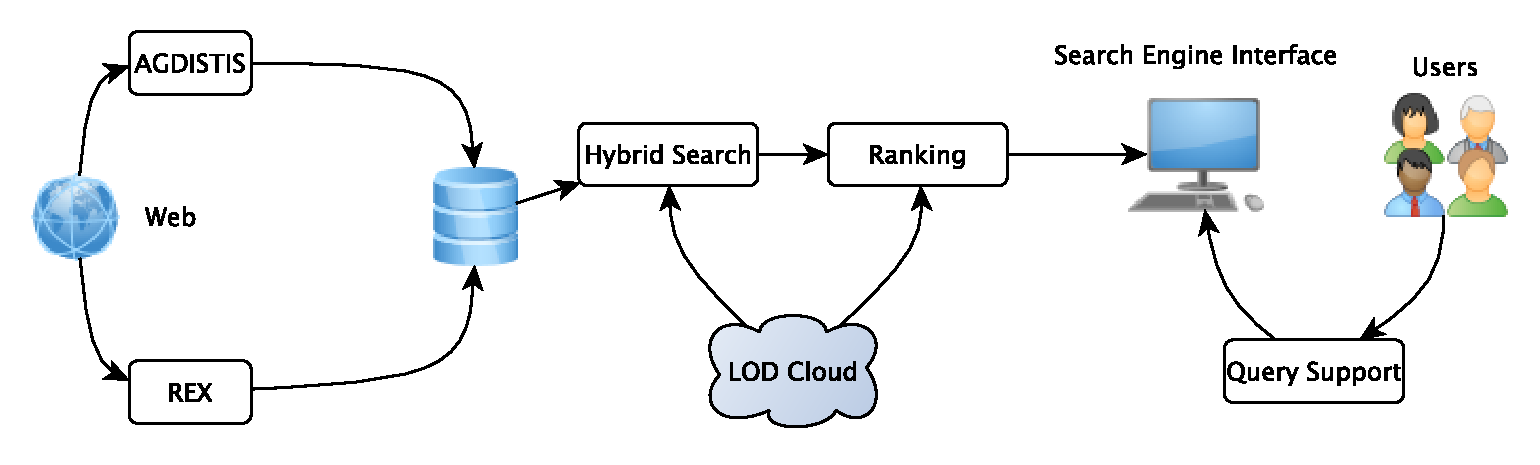
\includegraphics[width=\linewidth]{chapter_one/overview.pdf}
    \caption{Overview of the proposed information system architecture.}
    \label{overview}
\end{figure*}

The starting point of the proposed architecture is a two-fold data acquisition strategy based on a highly efficient, state-of-the-art industry Web crawler provided by our research partner \emph{Unister GmbH}.  

First, \emph{unstructured Web pages} from the crawled dataset, e.g., provided texts from news portals or agencies, are annotated by a standard NER algorithm~\cite{stanford} followed by a novel NED approach AGDISTIS~\cite{AGDISTIS}.
This NED approach has been developed to support arbitrary Linked Data knowledge bases to ensure future developments.
Moreover, AGDISTIS uses several NLP techniques to identify a set of candidate entities and identifies the correct with the help of the graph-based HITS algorithm. % and the resulting authority scores.
To prove the quality of AGDISTIS' results several corpora have been generated, evaluated and published. 
These corpora, called $N^3$~\cite{n3}, use the state-of-the-art serialization format \emph{NIF}~\cite{NIF} following the ``eating our own dogfood'' paradigm inherent to the Semantic Web community. 
$N^3$ are expected to form a novel gold standard in the areas of semantic named entity recognition and disambiguation.
Using $N^3$ and other well-known datasets, AGDISTIS has been proven to outperform the state-of-the-art algorithm AIDA~\cite{AIDA} by up to $16\%$ F-measure.
In the future, AGDISTIS will be evaluated against the framework of Cornolti et al.~\cite{cornolti} to provide a more comprehensive evaluation. 

Second, \emph{templated Web pages}, e.g., \url{http://www.imdb.com}, have been identified as another important source for answering user searches.
Therefore, REX~\cite{REX} has been developed during the early stage of this PhD work.
It is a web-scale semantic relation extraction framework capable to identify known as well as novel relations on Web pages creating RDF out of them.
REX combines a well-known wrapper induction technique~\cite{Crescenzi2013} for extracting XPath expressions, AGDISTIS as its NED algorithm and a consistency checker for the extracted relations based on ad-hoc generated schemas.
It has been shown that REX is able to generate new Linked Data triples with a precision of above $75\%$~\cite{REX}.

The resulting data from both pre-processing steps will serve as the underlying dataset for future research steps together with knowledge from the LOD Cloud.

Concerning the users' need for exploring the data space, %by enabling searches via keywords, natural language or even questions 
the next step is to \emph{support the formulation of queries}.
A huge potential within classical search engines is contained in inexact search queries, e.g., in terms of given a description only or a question.
Standard search engine methodologies fail at this point due to not being able to match keyword queries. 
In this thesis, we will support query formulation by providing on-the-fly recommended queries based on the real-time user input.
It is planned to use Linked Data such as \emph{BabelNet}\footnote{\url{http://babelnet.org/}} to find polysemes and synonyms within a query and thus enhancing the understanding of what the users actually mean.
Furthermore, three different standard approaches as well as a Linked Data-based grammar will be compared and evaluated against each other.
Another by-product of an according auto-completion approach is to teach the user which queries a search engine understands.

The research field of information retrieval/search and ranking has so far only been analysed theoretically within this doctoral work. 
In this thesis, a hybrid search engine is going to be implemented, i.e., an engine comprising a full-text information retrieval system enhanced by extracted Linked Data and a stake of LOD Cloud-based entity search.
Especially, the keyword-based search engine \emph{SINA}~\cite{sina} will be a starting point for further research. 

With respect to ranking algorithms, this PhD work focuses on two different research plans.
At first, a semantic extension of graph-based authority calculating algorithms will be investigated. 
Therefore, a master thesis has been looked after which analysed a context-driven enhancement of Stoyanovich's work~\cite{Stoyanovich}.
Initial results show an improvement compared to the baseline using the plain PageRank algorithm.
In parallel, an ensemble learning approach of Semantic Web-based ranking algorithms will be evaluated.

To summarize, the aforementioned steps will help building an integrated information system leveraging search engine performance using Linked Data.
Additionally--due to strong industry needs--this framework is going to be used in a real-life environment with web-scale amounts of users.
Finally, most of the source code will be published as open source and can be downloaded via the projects homepage\footnote{\url{http://aksw.org/RicardoUsbeck}}.

\section{Evaluation Plan and Conclusion}\label{conclusion}
This PhD work is dimensioned for three years. 
After intense literature reviews in the beginning of the first year the need for annotated Web data has been identified.
As a logical consequence, the development of AGDISTIS and REX had been finished by the end of the first year. 
Alongside, a gold standard ($N^3$) has been created to be able to evaluate the approaches mentioned above.

The second year will be used for developing and assessing the corresponding search and ranking procedures. 
To measure the quality of the \emph{auto-completion} technology, we assess different real-world query logs from our industry partner.
Thereby, we analyze how much characters are need to understand the query correct.
Additionally, we focus on the efficiency of the system in terms of milliseconds to react on a pressed key.

Considering the ranking evaluation, we will use standard precision, recall and f-measures as well as rank comparision measures, e.g., mean reciprocal rank. 
The underlying data is provided by the industry partner through human rater assessments and several comparisons to real-life search engines, e.g., Google or Wolfram Alpha.

Afterwards, the combined pipeline itself will be evaluated in a qualitative study using professionals and end users.
Therefore, empirical methods like Likert-scale questionnaires and direct relevance feedback will be used.


Next to refining already submitted work and optimizing the source code to meet industrial production standards, the developed approaches and algorithms will be refined in a spiral way if unpredictable results occur.
Thereby, upcoming ideas will be interweaved with the presented schedule creating a closed loop consisting of research question, development, evaluation and new research questions.

\chapter{Preliminaries}

%\begin{abstract}
Linked Data is becoming an increasingly popular method to publish data.
It is based on a simple set of rules and a number of widely adopted standards.
This introductory article aims at capturing the simplicity of Linked Data, and the concepts behind the related standards.
It will help the reader to understand the basic elements of Linked Data and its related technologies.
Using the example of a calendar app, we will highlight the practical advantages of using Linked Data for writing apps and publishing data in a completely decoupled way.
%\end{abstract}


\section{Introduction}
\label{intro}
Linked Data is a method to publish data on the Web, so that it can be connected to other datasets and create a Web of Data.
Four rules need to be followed in order to publish data as Linked Data~\cite{linkeddata-rules}:

\begin{enumerate}
\item Use URIs to name things
\item Use HTTP URIs so that they can be looked up
\item On lookup, provide useful information in standard formats
\item Provide links to other things
\end{enumerate}
%\todo[inline]{Was ist mit einer offenen Lizenz? Siehe 5 star data}

This chapter will describe the standards around Linked Data and their basic concepts.
Instead of focusing on completeness and technical correctness, we want to achieve an intuitive understanding in the interested but so far uninformed reader.
We refer to more comprehensive primers and the technical specifications in each section, so that the reader interested in more details can further deepen their knowledge.

Prerequisites for this chapter are merely a basic understanding of how the Web works.
It would be helpful if the reader was exposed to some basic ideas from data management, data structures, and knowledge representation.

Throughout the chapter we will use the example of writing a calendar application.
Our app will be able to deal with different time zones:
if the user enters a meeting like \textit{"Meeting at 9am in Atlanta"} the calendar tool should be able to translate the time to the local time zone, even if the meeting is being entered in Istanbul and shared with participants in Athens.

The chapter is structured as follows:
Section~\ref{semanticweb} explains the connection between Linked Data and the Semantic Web Vision.
Section~\ref{rdf} introduces the basic notions of RDF, especially the idea of an RDF graph and RDF triples.
Section~\ref{uri} describes URIs, the basic building blocks for such triples, and how they refer to the Web.
Section~\ref{http} then discusses how the Web is used for the distributed publishing of knowledge using the HTTP standard.
Secton~\ref{rdfs} extends the very simple expressivity of RDF, and discusses how languages like RDFS, OWL, and RIF are layered on top of it.
Section~\ref{sparql} introduces SPARQL, a query language for RDF graphs.
In Section~\ref{rdfa} we then go into more detail about the question how RDF is and can be serialized,
before we devote Section~\ref{xml} to the sometimes confusing relationship of RDF and XML.
We close in Section~\ref{conclusions} with a resum\'{e} on the state of Linked Data and an outlook on current developments.

\section{Vision of the Semantic Web}
\label{semanticweb}

Linked Data and \emph{Semantic Web} are sometimes used synonymously, although these two are rather different concepts.
The Semantic Web~\cite{semanticWeb} is a movement from the \texttt{Web of Documents} to the \texttt{Web of Data}.
The intention is to develop a Web that enables humans as well as machines to interact and work on existing data in way that creates an additional value.
To achieve this the data needs to be machine understandable, human manageable, linkable and storable in a standardized way.
Linked Data is the materialized implementation of the Semantic Web vision, executed by technologies like RDF, SPARQL, ontologies and many more decribed below.

\medskip

\textbf{Further readings}:
To get to know more about the Semantic Web vision we refer to the book~\cite{swbook} or the W3C Semantic Web website at \url{http://www.w3.org/standards/semanticweb/}.

\section{RDF: The basics}
\label{rdf}

RDF is a standardized model used for representing knowledge on the Web.
Knowledge representation in general enables to separate what a system does from what it knows~\cite{brachmannKR}, i.e., to make its knowledge explicit and not simply implicit in the program.
Decoupling knowledge from a program has several advantages, for example, it allows the knowledge base to be maintained externally, so that changes in the world may not even affect the code.

In the calendar app, one approach to deal with the different time zones would be to code the information into the program itself. 
We could simply have a function that, given a country or city name, returns the offset, implemented with a lot of \texttt{switch} or \texttt{if then else} statements.
A change in the timezone of a country would require rewriting the function and recompiling the whole application.
Instead, we could externalize the knowledge about countries and cites and their time zones.
The application would then load the knowledge base whenever it is needed, and behave accordingly.

There are many different ways to represent the knowledge in a way that the application can read it.
For example, we could have a database with tables of cities and countries and associated time zones.
We could have comma separated lists of cities for each time zone.
Or we could gather a consortium and define a standard for expressing time zone information, so that different developers can independently access this knowledge in their apps.%
\footnote{For time zones, this is roughly what happened, in form of the \textit{tz database}.}

RDF provides a generic, standardized model for representing knowledge.
Generic means, that it can be used in any domain, be it time zones, geographic data, genes, books, or anything else.
Standardized means that RDF has been specified in an explicit, reimplementable way, so that everyone can create software that can correctly read and write RDF documents.

The basic notions of RDF are triples and graphs.
Triples are used to express the given knowledge, piece by piece.
Each triple is built of three elements: a subject, a predicate, and an object.
In our example, a piece of knowledge could be expressed with the following triple:

\begin{verbatim}
 Turkey timezone EET .
\end{verbatim}

The subject in this triple is \texttt{Turkey}, the predicate is \texttt{timezone}, and the object \texttt{EET}.
The triple can intuitively be understood as having the same meaning as the English sentence \textit{"Turkey is in the timezone EET."}.

A graph consists of a set of triples.
It is called a graph, because the subjects and objects can be understood as nodes, connected with directed edges labeled with the given property.
The following example graph is visualized in Figure~\ref{fig:graph}.
\begin{verbatim}
 Turkey timezone EET .
 Greece timezone EET .
 Georgia timezone GET .
 EET borders GET .
 EET offset "2"^^int .
 GET offset "4"^^int . 
\end{verbatim}

\begin{figure}
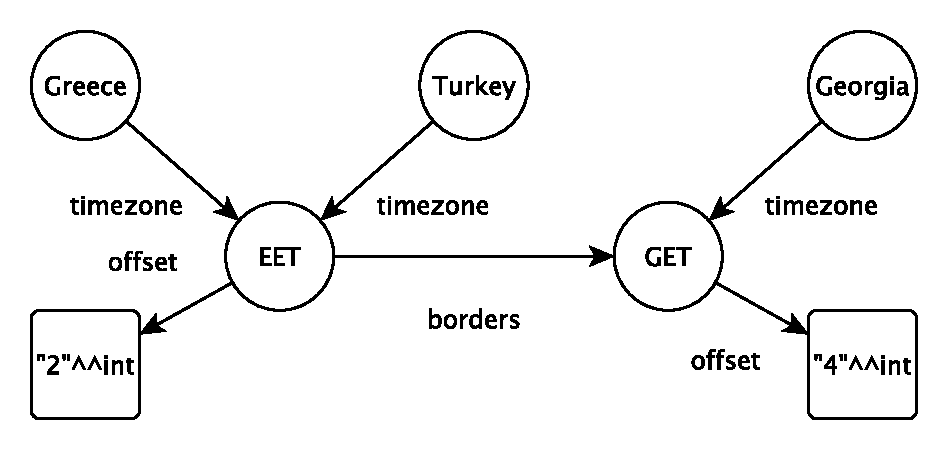
\includegraphics[width=\linewidth]{chapter_two/fig_graph.pdf}
\caption{Example of Linked Data used for the calender application}
\label{fig:graph}
\end{figure}

The last two triples in the example graph demonstrate the use of literal values in the object position: instead of a named node, that refers to an entity, we have a typed literal value.
The type in this case is \texttt{int}, which means that the values should be interpreted as integers.
The types available in RDF cover numbers, strings, booleans, dates, time durations, URIs, XML, and others.

\medskip

\textbf{Further readings}:
If you want to get deeper into the formalisms behind RDF have a look at the the RDF specification~\cite{rdf-spec}, 
the RDF primer~\cite{rdf-primer}, 
the specification for XSD datatype~\cite{xsd-part2}.
Relevant concepts we did not introduce are blank nodes, reification, named graphs and extensible datatypes~cf.~\cite{ namedgraphs,rdf-primer}.

\section{URIs: The words of the language}
\label{uri}

The big advantage of a graph-based model is that they can be easily be merged, by simply regarding a merger as a union of the triples in both graphs.
Many other models for knowledge representations, like tables or XML files, do not allow for such a generic merging.
But in order to provide a knowledge representation language that allows these kind of mergers, naming conflicts must be avoided.
In our example, \texttt{Georgia} refers to the caucasian country.
But now consider a second knowledge base about US states:

\begin{verbatim}
 Georgia timezone EST .
 SouthCarolina timezone EST .
 EST offset "-5"^^int .
\end{verbatim}

Since both Georgias -- the caucasian country and the US state -- are named the same, we would not be able to differentiate them.
Georgia now seems to be both in the timezone \texttt{GET} and \texttt{EST}!

To avoid this situation, all entities in Linked Data have to be referred to by unique names.
To achieve this, the names are given as URIs, most often HTTP URIs (just like websites).
The advantage of URIs is that anyone can register a prefix, and then create new names with this prefix.
The owner of the prefix is responsible for what the given name means.
So, the country Georgia could be named \texttt{http://example.org/countries\#Georgia} and the us state could be \texttt{http://example.org/usstates\#Georgia}.
As long as everyone defines new names in their own namespace only, naming conflicts can be avoided without constant coordination between all parties.

As URIs can be quite lengthy, often qualified names (or \textit{QNames}) are used.
They have the form \texttt{prefix:localName}.
Prefixes are defined locally to expand to a certain namespace, e.g., in our example we could define that the prefix \texttt{us} means the namespace \texttt{http://example.org/usstates\#}, and thus we could use the qualified name \texttt{us:Georgia} in order to refer to the complete URI \texttt{http://example.org/usstates\#Georgia}.

\medskip

\textbf{Further readings}:
To find more about the specification of URIs, see~\cite{uri} and for to get to know how to register a new URI scheme, have a look at~\cite{uri-registration}.
We did not speak about IRIs~\cite{iri} and other protocols besides HTTP, like FTP~\cite{ftp} or URN~\cite{urn}.

\section{HTTP: Distributed knowledge}
\label{http}

The second rule for publishing linked data is to use HTTP URIs.
The advantage is, that HTTP is a widely implemented protocol, that can be used over the Internet for accessing resources with a given HTTP URI.
For example, the above knowledge base could have itself the name \texttt{http://example.org/countries}.
Now a simple HTTP \texttt{GET} command like

\begin{verbatim}
 GET http://example.org/countries
\end{verbatim}

will return the knowledge base (it can be tried by entering the URI in a browser, but it is suggested for later as the result might be confusing at this point).

All entities are named with URIs, and the third rule of Linked Data asks to return information about the entity identified with a given URI when the URI is being dereferenced via HTTP.
This way, the Web can be used as vast knowledge space, where everyone can publish what they know about a given entity.

We can also use the URIs of others -- we do not have to publish URIs for all entities that we want to use ourselves.
For example, DBpedia is a widely used resource that publishes Linked Data based on Wikipedia's infoboxes~\cite{dbpedia}.
DBpedia offers URIs for all entities that have a Wikipedia page.
For example, Greece' Wikipedia page is \texttt{http://en.wikipedia.org/wiki/Greece} and, based on that, DBpedia defines the URI for Greece to be \texttt{http://dbpedia.org/resource/Greece}.
If this is entered into a browser, the browser redirects the user to a Web page about Greece in DBpedia.
If a Semantic Web application would have asked, DBpedia (prefix dbpedia) would have returned the RDF data instead.

So we could replace

\begin{verbatim}
 countries:Greece tz:timezone tz:EET .
\end{verbatim}

with using the DBpedia URI for Greece and get

\begin{verbatim}
 dbpedia:Greece tz:timezone tz:EET .
\end{verbatim}

This would have the advantage that now we can learn much more about Greece: the name of the country in different languages and alphabets, its population, the name of the head of state, etc.
Suddenly, our application can use knowledge from all over the Web.

Instead of simply replacing the URI, in our case we actually state that the URIs refer to the same entity, like this:

\begin{verbatim}
 countries:Greece owl:sameAs dbpedia:Greece .
\end{verbatim}

We see, that also properties can be reused from all over the Web.
In this case we use the term \texttt{sameAs} from the OWL vocabulary, which we will look at in the next section.

One advantage of using the Web as a knowledge base is that much knowledge is already published:
whereas our knowledge bases had information on some countries, Websites like Geonames or DBpedia offer lists of cities, and in which countries or US states they are located.
So regarding the cities we mentioned in the beginning of the article, the Web already offers the following pieces of knowledge:

\begin{verbatim}
 dbpedia:Istanbul dbo:country dbpedia:Turkey .
 dbpedia:Athens dbo:country dbpedia:Greece .
 dbpedia:Atlanta dbo:isPartOf dbpedia:Georgia_(U.S._state) .
\end{verbatim}

This allows us to just reuse the knowledge about cities from the Web of Data, for very little cost.

\medskip

\textbf{Further readings}:
For a deeper introduction of the HTTP protocol have a look at the HTTP specification~\cite{http}.

\section{RDFS, OWL and others: Adding expressivity}
\label{rdfs}

RDF allows us to express triples directly.
A very powerful method is to allow for implicit triples, by using more expressive semantics than simple triples.
We have seen one example already: \texttt{owl:sameAs} states that two URIs refer to the same entity.
That means that anything we say about \texttt{dbpedia:Greece} is also true about \texttt{countries:Greece}.
So now that we learnt that \texttt{dbpedia:Athens} is in \texttt{dbpedia:Greece}, we know that it is also in our own \texttt{countries:Greece}.

A number of languages build on top of RDF and extend it with more expressive semantics.
We will look at three of them, that are standardized by the W3C: RDFS, OWL, and RIF.

RDFS is the simplest one of them.
It allows us to describe class and property hierarchies:
for example, we have found on the Web cities connected to countries resp. US states.
The connection to the country was done using the \texttt{dbo:country}, to the state with \texttt{dbo:isPartOf}.
Now we can also define that everything that is connected via the former should also be connected through the latter.
In RDFS we do that with the following triple:

\begin{verbatim}
 dbo:country rdfs:subPropertyOf dbo:isPartOf .
\end{verbatim}

Now a reasoner who follows the RDFS semantics can infer that

\begin{verbatim}
 dbpedia:Istanbul dbo:isPartOf dbpedia:Turkey .
\end{verbatim}

is true, even though it was never stated explicitly.

OWL is much more expressive regarding the description of classes and properties:
for example, we can state that every city has to be in exactly one time zone, or that nothing can be both a U.S. state and a country, which could have helped to discover the error with the two Georgias automatically.

Since RDF allows only triples, such more complex statements need to be broken down to triples.
The statement \textit{"Every city is in exactly one time zone."} translates in RDF to the following four triples:

\begin{verbatim}
x:statement1 rdf:type owl:Restriction .
x:statement1 owl:onProperty tz:timezone .
x:statement1 owl:qualifiedCardinality "1"^^xsd:nonNegativeInteger .
x:statement1 owl:onClass dbo:City .
\end{verbatim}

Although this might seem a bit daunting, in reality these kind of triples are hidden either by more high-level syntaxes (see Section~\ref{rdfa}) or query tools (see Section~\ref{sparql}).

RIF is a different beast.
Whereas OWL is an expressive language to describe classes and properties, RIF is a way to express rules of them form \textit{if\ldots{}then\ldots{}}.
In our example, we might want to state that whenever a city is part of a country or state, and the country or state has a time zone, this is also the time zone of the city. Or, using the variables \texttt{?x}, \texttt{?y}, and \texttt{?z}:%
\footnote{We will not show how the rule is represented in RDF, as this looks even worse than the OWL statement above.}

If
\begin{verbatim}
 ?x dbo:isPartOf ?y .
 ?y tz:timezone ?z .
\end{verbatim}
then
\begin{verbatim}
 ?x tz:timezone ?z .
\end{verbatim}

RDFS, OWL, and RIF can, at least in theory, be all used together.
It depends on the used tools if a given semantics is understood: some reasoners support parts of OWL (so called fragments), some support only RDFS, other RIF, and a very few claim to support interesting combinations of all three languages, and sometimes beyond.

\medskip

\textbf{Further readings}:
The whole formalism can be found in the specifications for RDFS~\cite{rdfs}, OWL~\cite{owl}, and RIF~\cite{rif},but especially at the OWL primer in this book~\cite{dl-primer}.
We did not discuss questions of how to reason and about the complexity and decidability of reasoning. 
This is a big research topic, and in the last few years, it was advanced tremendously. 
We point to the DL Handbook as an entry point into this topic~\cite{dl-handbook}.
We also did not mention the different fragments of OWL, RIF, and the differences between OWL and OWL2, which can all be found in detail in the respective standards.
Besides the languages presented here, other languages like SKOS~\cite{skos} or WSML~\cite{wsml} exist, that can define other semantics.

\section{SPARQL: Querying RDF}
\label{sparql}

So far, we have described how to express knowledge: both simple facts (with RDF) and more expressive statements that enrich the knowledge base (in the previous section).
SPARQL provides a query language for RDF knowledge bases.

For example, assume that we have all the triples we have mentioned so far in one graph that we can query via SPARQL.
Let's also assume that the system providing the SPARQL endpoint understands the semantics of RDFS, OWL, and RIF.
Now we can ask for the offset for Athens:

\begin{verbatim}
 SELECT ?offset WHERE {
   dbpedia:Athens tz:timezone ?tz .
   ?tz tz:offset ?offset .
 }
\end{verbatim}

The system will return as a result the integer $2$.

Athens is in the country Greece. We know that from the Web.
Due to the OWL subproperty triple, we also know that to be in a country means to be part of it.
Because of the RIF rule, we can infer that if something is part of something, it also has the same timezone.
Based on this, the following two triples, the first one implicit, the second given explicitly, are in our knowledge base:

\begin{verbatim}
 dbpedia:Athens tz:timezone tz:EET .
 tz:EET tz:offset "2"^^xsd:int .
\end{verbatim}

A SPARQL query describes a triple pattern (similar to the one in the \textit{if}-part of RIF),
where symbols with a leading question mark are variables.
A SPARQL processor now tries to find values for the variables, so that the whole SPARQL pattern can be fulfilled by the knowledge base.
The SPARQL processors then returns a list of all possible answers for the selected variables,%
\footnote{That is, all variables following the introductory \texttt{SELECT} keyword, in this case \texttt{?offset}.}
i.e. in this case for all values that \texttt{?offset} can have so that the SPARQL query pattern matches in the knowledge base.
Given our query pattern, the two triples above are the only match in our knowledge base, and thus the result, \texttt{"2"\texttt{\char`\^}\texttt{\char`\^}xsd:int } will be returned as the only possible value for \texttt{?offset}.

SPARQL can be regarded as the main interface to access knowledge on the Web of Data.
Currently, the usual workflow to work with Linked Data is to find and gather trustworthy data from the Web, include some knowledge created for the task or tying together the data from the Web, put it all in one knowledge base, and then use SPARQL to get answers to the queries of interest to the given task.

\medskip

\textbf{Further readings}:
To find out more about SPARQL look at the specification for SPARQL~\cite{sparql}.
We did not discuss that SPARQL is not only a query language but also a protocol of how to acccess SPARQL endpoints.
We also did not discuss other types of queries: \texttt{DESCRIBE}, \texttt{ASK}, and \texttt{CONSTRUCT}, nor the powerful features of SPARQL to count, do math, regular expressions, named graphs, etc.

\section{RDFa and Co.: Serializations of RDF}
\label{rdfa}
What is a serialization?
To send around RDF graphs through the Web, we need somehow to write them down in documents, i.e. to serialize them in a sequence of tokens.
Throughout this chapter we have used a slightly simplified, triple-based serialization, N3~\cite{n3}.
N3 has the advantage, that the triple structure of the graph is very obvious.
Although, it is widely used, it has the disadvantage of not being standard.

There are a confusing number of serializations of RDF around, mostly due to the fact that the orginally standardized serialization in RDF/XML is considered to be not very pleasing.
Soon, further syntaxes were created, some of them also in XML (like TriX~\cite{trix}), some of them not (like N3 and its constrained version N-Triples~\cite{ntriples}.
Expressions in other languages like OWL and RIF were often very cumbersome to be translated to RDF (as shown in Section~\ref{rdfs}), and thus introduced serializations of their own, like the OWL Functional Syntax~\cite{owl2}, the OWL XML presentation syntax (a serialization of OWL directly in XML, instead of going through RDF~\cite{owl3}), the RIF syntaxes~\cite{rif}, etc.
Lately, JSON became a more prominent serialization format on the Web, and standards to represent the RDF data model in JSON are being worked on~\cite{json-ld}.

Besides serializations for pure RDF, there has been a second strand of embedding RDF in other file formats.
One of the main use cases for RDF is to provide flexible metadata about a file.
Embedding that metadata in the file itself has the advantage that the metadata is easier retained if the file gets moved, shared, changed, etc.
A growing number of file formats, like Adobe's (PDF, Photoshop, etc.) allow to embed RDF~\cite{xmp}.

The most relevant file format for the Web is obviously HTML itself, the language to describe Web pages and applications.
The RDFa standard offers how to markup and annotate elements of a Web page with RDF.
This allows a tool understanding RDFa to directly extract structured data out of a Website:
a page about an event can be pulled into a calendar,
a restaurant can be automatically filtered with the allergies of the user,
different shopping Websites can be thrown into one knowledge base and be compared directly, etc.

\medskip

\textbf{Further readings}:
If you want to find more serializations have a look at the specifications of RDFa~\cite{rdfa}, RDF in JSON~\cite{json-ld}, and RDF/XML~\cite{rdfxml}.
Also relevant is the ongoing conversation between the communities supporting Microformats~\cite{microformats}, Microdata~\cite{microdata}, and RDFa.

\section{XML: The confusing older brother}
\label{xml}

XML became the de-facto lingua france for data on the Web and beyond.
So it was natural, that it was assumed that RDF would be build on top of XML.
But in reality, the two are very different beasts:
XML describes a tree-based model, with a single root element, that has child elements in a strict order, and, who in turn, might have further child elements, in strict orders too, all strictly hierarchical.
RDF describes a graph-based model, where the order of the edges does not matter, and that is expressed as a simple set of triples.
XML schema defines a strict grammar for the elements in an XML documents, determining if an XML file is valid or not.
RDF schemas provide additional knowledge to infer implicit knowledge from a given RDF file, and can hardly be used to check the validity of an RDF file.
It is often easier to deal with valid XML files than with RDF files, because the developer has guarantees about the structure of the file.
On the other hand, RDF files are much easier to extend: one can simply add further triples, and, as long as they don't contradict the existing triples, the knowledge simply grows.
Two RDF files can always be simply merged automatically. For XML files in general, such an operation makes no sense.

With the benefit of hindsight, forcing RDF into an XML-based serialization was bound to lead to numerous problems without gaining the hoped-for advantages.
Many of the existing XML tools and workflows were actually unable to deal with RDF/XML files, so that the existing huge pool of experience and software could not be used to kickstart the Web of Data.

Today, XML does not play a prominent role for the Web of Data anymore.
Even if it gets further used as the main serialization format for RDF, its data model and the tools used with XML are loosing relevance.
It is an open question if this might change again, or if the rich set of software and experiences surrounding the XML world can be unlocked in favor of the Web of Data -- or the other way around.

\medskip

\textbf{Further readings}:
For more information about XML, see the XML specification~\cite{xml} or the XML Schema primer~\cite{xml-primer}.

\section{Conclusions and outlook}
\label{conclusions}

RDF is increasingly becoming the standard way to share data on the Web.
Using and publishing RDF is not an academic exercise anymore.
The flexibility and extensibility of RDF, together with the possibility to merge arbitrary RDF graphs, gives it a unique advantage compared to other wide spread data models.
Confusions surrounding its several serializations, especially the ill-received standard RDF/XML-serialization, a maybe too early focus on OWL, and the late availability of SPARQL, have probably hampered uptake.
Meanwhile, simple standards like Microformats and JSON have received considerable uptake.

The advantages and the genericity of Linked Data standards are being increasingly recognized.
Instead of introducing hundreds, if not thousands of APIs and heterogeneous formats, one common data model and query language can substantially decrease costs of data integration and data reuse.

End user interfaces to the Web of Data are still missing -- but maybe they always will.
Maybe the role of Linked Data is to be background technology:
no one asks for generic interfaces for end-users to SQL databases.
Maybe the Web of Data has a similar fate.

Still several practical issues remain unresolved:
\begin{itemize}
\item In general, SPARQL is too powerful and too expensive for the Web. It is far too easy to bring a SPARQL endpoint down with a few queries.
\item The multitude of serialization formats in practical use combined with the lack of standard formats besides RDF/XML hampers teaching about RDF and its uptake.
\item For a number of wide-spread use cases, no standards or even widely acknowledged best practices exist: how to express numbers with units, especially imperial units? How to express data that was valid at a given point in time? How to express time spans? How to deal with numerical precision? How to work with simple geographical and temporal reasoning, like inclusion?
\item The current standards allow fine-grained provenance information only through reification, a method, that is often strongly discouraged for several reasons.
\item The semantics break down under inconsistencies. There is currently no accepted way to deal with diversity in knowledge bases, even though this will play a crucial role on the Web. This ties in with questions of trust that have not yet been sufficiently tackled: given diverse data about an entity, maybe even contradictions, how to choose which sources to trust? How to make this trust transferable to the user?
\end{itemize}

The Web of Data, as part of the Web, is getting increasingly tangled with all aspects of our lives.
The growing number of intelligent apps and devices in our environment will have an ever-growing need to communicate with each other.
Imagining a future where our calendar app can support the flight finder app by restricting the departure and arrival times based on our agenda and the locations of our meetings and the airport, has become much easier today than it used to be only a few years ago.
Such a future is much easier to achieve when the applications and devices can all communicate in the same common and standard data model, and using the same interfaces.





\part{Knowledge Extraction from Unstructure Data}
\cleardoublepage
\ctparttext{
    The second part 
}
\newmdtheoremenv{ex}{Example}

\chapter{Knowledge-base Agnostic, Multilingual Entity Linking}
%\begin{abstract}
Over the last decades, several billion Web pages have been made available on the Web.
The ongoing transition from the current Web of unstructured data to the Web of Data yet requires scalable and accurate approaches for the extraction of structured data in RDF (Resource Description Framework) from these websites.
%Web/news data (WND) is the largest growing source of dynamic information on the Web outlining its importance in the upcoming Web of Data. 
One of the key steps towards extracting RDF from text is the disambiguation of named entities.
While several approaches aim to tackle this problem, they still achieve poor accuracy. % which is a permanently growing source of up-to-date information at the Web.
We address this drawback by presenting AGDISTIS, a novel knowledge-base-agnostic approach for named entity disambiguation.
Our approach combines the Hypertext-Induced Topic Search (HITS) algorithm with label expansion strategies and string similarity measures.
Based on this combination, AGDISTIS can efficiently detect the correct URIs for a given set of named entities within an input text. 
We evaluate our approach on eight different datasets against state-of-the-art named entity disambiguation frameworks.
%Moreover, we present an extension based on topic modeling which improves the quality of the extraction in difficult cases by up to $3\%$.
Our results indicate that we outperform the state-of-the-art approach by up to $29\%$ F-measure.
%\end{abstract}

\section{Introduction}
The vision behind the Web of Data is to provide a new machine-readable layer to the Web where the content of Web pages is annotated with structured data (e.g., RDFa~\cite{rdfa}).
However, the Web in its current form is made up of at least 15 billion Web pages.\footnote{Data gathered from \url{http://www.worldwidewebsize.com/} on January 4th, 2014.}
Most of these websites are unstructured in nature.
Realizing the vision of a usable and up-to-date Web of Data thus requires scalable and accurate natural-language-processing approaches that allow extracting RDF from such unstructured data.
Three tasks play a central role when extracting RDF from unstructured data: named entity recognition (NER), named entity disambiguation (NED), also known as entity linking~\cite{Mihalcea:2007:WLD:1321440.1321475}, and relation extraction (RE).
For the first sentence of Example~\ref{ex:obama}, an accurate named entity recognition approach would return the strings \texttt{Barack Obama} and \texttt{Washington, D.C.}.
A high-quality DBpedia-based named entity disambiguation (NED) approach would use these already recognized named entities and map the strings \texttt{Barack Obama} resp. \texttt{Washington, D.C.} to the resources \texttt{dbr:Barack\_Obama} and \texttt{dbr:Washington,\_D.C.}\footnote{\texttt{dbr:} stands for \url{http://dbpedia.org/resource/}}~\cite{dbpedia-swj}.
\begin{ex}
Barack Obama arrived this afternoon in Washington, D.C.. President Obama's wife Michelle accompanied him.
\label{ex:obama}
\end{ex}
While NER has been explored extensively over the last decades~\cite{StanfordNER}, the disambiguation of named entities,\,i.e., the assignment of a resource's URI from an existing knowledge base to a string that was detected to label an entity remains a difficult task.

Current NED approaches suffer from two major drawbacks:
First, they poorly perform on Web documents~\cite{RatinovRo09}.
This is due to Web documents containing resources from different domains within a narrow context.
An accurate processing of Web data has yet been shown to be paramount for the implementation of the Web of Data~\cite{GER+13}.
%, Web data is a very worthwhile source of latest information which is often not yet captured in any knowledge base. 
Well-know approaches such as \emph{Spotlight}~\cite{spotlight} and \emph{TagMe 2}~\cite{TagMe2} have been designed to work on a particular knowledge base.
However, Web data contains resources from many different domains.
%Ttha named entity disambiguation framework has to be able to work on any knowledge base in order to capture content from different domains.
Hence, we argue that NED approaches have to be designed in such a way that they are agnostic of the underlying knowledge base.
%Being capable of using specialized or language-specific knowledge bases should lead to high F-measures. 
Second, most state-of-the-art approaches rely on exhaustive data mining methods~\cite{Cucerzan07,rat:rot} or algorithms with non-polynomial time complexity~\cite{Kleb11WIMS}.
However, given the large number of entities that must be disambiguated when processing Web documents, scalable NED approaches are of central importance to realize the Semantic Web vision.
%\todo[inline]{Micha: The sentence "Hence, we argue that NED..." is not really good. From my point of View it sounds like "A NED-algorithm has to use more than one KB at the same time".}

In this paper, we address these drawbacks by presenting AGDISTIS, a novel NED approach and framework.
AGDISTIS achieves \emph{higher F-measures} than the state of the art while remaining \emph{polynomial in its time complexity}.
AGDISTIS achieves these results by combining the HITS algorithm~\cite{HITS} with label expansion and string similarity measures.
Overall, our contributions can be summed up as follows:
(1) We present AGDISTIS, an accurate and scalable framework for disambiguating named entities that is agnostic to the underlying knowledge base (KB) and show that we are able to outperform the state of the art by up to $29\%$ F-measure on these datasets.
%\todo[inline]{description of datasets? multilingual, multi-domain}
(2) We show that our approach has a quadratic time complexity. Thus, it scales well enough to be used even on large knowledge bases.
(3) We evaluate AGDISTIS on eight \emph{well-known and diverse open-source datasets}.\footnote{Further data, detailed experimental results and source code for this paper are publicly available on our project homepage \url{http://aksw.org/Projects/AGDISTIS}.} 

The rest of this paper is organized as follows: We first give a brief overview of related work in Section~\ref{sec:relatedwork}. 
Then, we introduce the AGDISTIS approach in Section~\ref{sec:approach}. %comprising an overview, the way AGDISTIS detects candidates and the disambiguation algorithm itself. 
%We formalize the task of NED in Section~\ref{sec:ned}.
After presenting the datasets, we evaluate our approach against the state of the art frameworks AIDA and TagMe 2 and the well-known DBpedia Spotlight. 
Furthermore, we measure the influence of using surface forms,\,i.e., synonymous label for a specific resource, in Section~\ref{sec:eval}. 
%\todo{surface form richtig erklärt?}
%We analyze the contribution of certain properties to our disambiguation approach in the same section. 
We conclude in Section~\ref{sec:conclusion} by highlighting research questions that emerged from this work.
%Our approach is open-source and can be found at \url{http://aksw.org/Projects/AGDISTIS}.
A demo of our approach (integrated into the Named Entity Recognition framework FOX~\cite{FOX}) can be found at \url{http://fox.aksw.org}. 


\section{Related Work}
\label{sec:relatedwork}
AGDISTIS is related to the research area of Information Extraction~\cite{nad:sek} in general and to NED in particular.
Several approaches have been developed to tackle NED. 
Cucerzan presents an approach based on extracted Wikipedia data towards disambiguation of named entities~\cite{Cucerzan07}.
The author aims to maximize the agreement between contextual information of Wikipedia pages and the input text by using a local approach.
%\todo{What's a local approach?}
\emph{Epiphany}~\cite{epiphany} identifies, disambiguates and annotates entities in a given HTML page with RDFa. 
Ratinov et al.~\cite{rat:rot} described an approach for disambiguating entities from Wikipedia KB. 
The authors argue that using Wikipedia or other ontologies can lead to better global approaches than using traditional local algorithms which disambiguate each mention separately using,\,e.g., text similarity. %for word sense disambiguation.
Kleb et al.~\cite{Kleb11WIMS,KlebESWC10} developed and improved an approach using ontologies to mainly identify geographical entities but also people and organizations in an extended version. 
These approaches use Wikipedia and other Linked Data KBs.
LINDEN~\cite{LINDEN} is an entity linking framework that aims at linking identified named entities to a knowledge base.
To achieve this goal, LINDEN collects a dictionary of the surface forms of entities from different Wikipedia sources, storing their count information.

Wikipedia Miner~\cite{milne2008learning} is the oldest approach in the field of \emph{wikification}.
Based on different machine learning algorithms, the systems disambiguates w.r.t. prior probabilities, relatedness of concepts in a certain window and context quality. 
The authors evaluated their approach based on a Wikipedia as well as an AQUAINT subset. 
Unfortunately, the authors do not use the opportunities provided by Linked Data like DBpedia.

Using this data the approach constructs candidate lists and assigns link probabilities and global coherence for each resource candidate.
The AIDA approach~\cite{AIDA} for NED tasks is based on the YAGO2\footnote{\url{http://www.mpi-inf.mpg.de/yago-naga/yago/}} knowledge base and relies on sophisticated graph algorithms. 
Specifically, this approach uses dense sub-graphs to identify coherent mentions using a greedy algorithm enabling Web scalability. 
Additionally, AIDA disambiguates w.r.t.~similarity of contexts, prominence of entities and context windows.

Another approach is DBpedia Spotlight~\cite{spotlight}, a framework for annotating and disambiguating Linked Data Resources in arbitrary texts.
In contrast to other tools, Spotlight is able to disambiguate against all classes of the DBpedia ontology.
Furthermore, it is well-known in the Linked Data community and used in various projects showing its wide-spread adoption.\footnote{\url{https://github.com/dbpedia-spotlight/dbpedia-spotlight/wiki/Known-uses}}
Based on a vector-space model and cosine similarity DBpedia Spotlight is publicly available via a web service\footnote{\url{https://github.com/dbpedia-spotlight/dbpedia-spotlight/wiki/Web-service}}.

In 2012, Ferragina et al. published a revised version of their disambiguation system called TagMe 2.
The authors claim that it is tuned towards smaller texts,\,i.e., comprising around 30 terms.
TagMe 2 is based on an anchor catolog (\texttt{<a>} tags on Wikipedia pages with a certain frequency), a page catalogue (comprising all original Wikipedia pages,\,i.e., no disambiguations, lists or redirects) and an in-link graph (all links to a certain page within Wikipedia).
First, TagMe 2 identifies named entities by matching terms with the anchor catalog and second disambiguates the match using the in-link graph and the page catalog via a collective agreement of identified anchors. 
Last, the approach discards identified named entities considered as non-coherent to the rest of the named entities in the input text.  

In 2014, Babelfy~\cite{babelfy} has been presented to the community.
Based on random walks and densest subgraph algorithms Babelfy tackles NED and is evaluated with six datasets, one of them the later here used AIDA dataset. 
In constrast to AGDISTIS, Babelfy differentiates between word sense disambiguation, i.e., resolution of polysemous lexicographic entities like \emph{play}, and entity linking, i.e., matching strings or substrings to knowledge base resources.
Due to its recent publication Babelfy is not evaluated in this paper.

Recently, Cornolti et al.~\cite{cornolti} presented a benchmark for NED approaches.
The authors compared six existing approaches, also using DBpedia Spotlight, AIDA and TagMe 2, against five well-known datasets. % on different tasks and with different measures.
Furthermore, the authors defined different classes of named entity annotation task, e.g. \emph{`D2W'}, that is the disambiguation to Wikipedia task which is the formal task AGDISITS tries to solve.
We consider TagMe 2 as state of the art w.r.t. this benchmark although only one dataset has been considered for this specific task.
We analyze the performance of DBpedia Spotlight, AIDA, TagMe 2 and our approach AGDISTIS on four of the corpora from this benchmark in Section~\ref{sec:eval}.

\section{The AGDISTIS Approach} 
\label{sec:approach}

\subsection{Named Entity Disambiguation}
\label{sec:ned}

The goal of AGDISTIS is to detect correct resources from a KB $K$ for a vector $N$ of $n$ a-priori determined named entities $N_1,\ldots,N_n$ extracted from a certain input text $T$.
In general, several resources from a given knowledge base $K$ can be considered as candidate resources for a given entity $N_i$.
For the sake of simplicity and without loss of generality, we will assume that each of the entities can be mapped to $m$ distinct candidate resources.
Let $C$ be the matrix which contains all candidate-entity mappings for a given set of entities.
The entry $C_{ij}$ stands for the $j^{th}$ candidate resource for the $i^{th}$ named entity. 
Let $\mu$ be a family of functions which maps each entity $N_i$ to exactly one candidate $C_{ij}$. 
We call such functions \emph{assignments}.
The output of an assignment is a vector of resources of length $|N|$ that is such that the $i^{th}$ entry of the vector maps with $N_i$.

Let $\psi$ be a function which computes the similarity between an assignment $\mu(C,N)$ and the vector of named entities $N$.
The \emph{coherence} function $\phi$ calculates the similarity of the knowledge base $K$ and an assignment $\mu$, cf. Ratinov et al.~\cite{rat:rot}, to ensure the topical consistency of $\mu$.
The coherence function $\phi$ is implemented by the HITS algorithm, which calculates the most pertinent entities while the similarity function $\psi$ is,\,e.g., string similarity.
Given this formal model, the goal is to find the assignment $\mu^\star$ with
\begin{equation*}
\mu^\star= \operatorname*{arg\,max}\limits_{\mu}\left(\psi(\mu(C,N), N) + \phi(\mu(C,N),K)\right).
\end{equation*}

The formulation of the problem given above has been proven to be NP-hard, cf. Cucerzan et al.~\cite{Cucerzan07}.
Thus, for the sake of scalability, AGDISTIS computes an approximation $\mu^{+}$ by using HITS, a fast graph algorithm which runs with an upper bound of $\Theta(k\cdot |V|^2)$ with $k$ the number of iterations and $|V|$ the number of nodes in the graph.
Furthermore, using HITS leverages 1) scalability, 2) well-researched behaviour and 3) the ability to explicate semantic authority. 

\subsection{Architecture}
\begin{figure*}[h!tb]
\centering
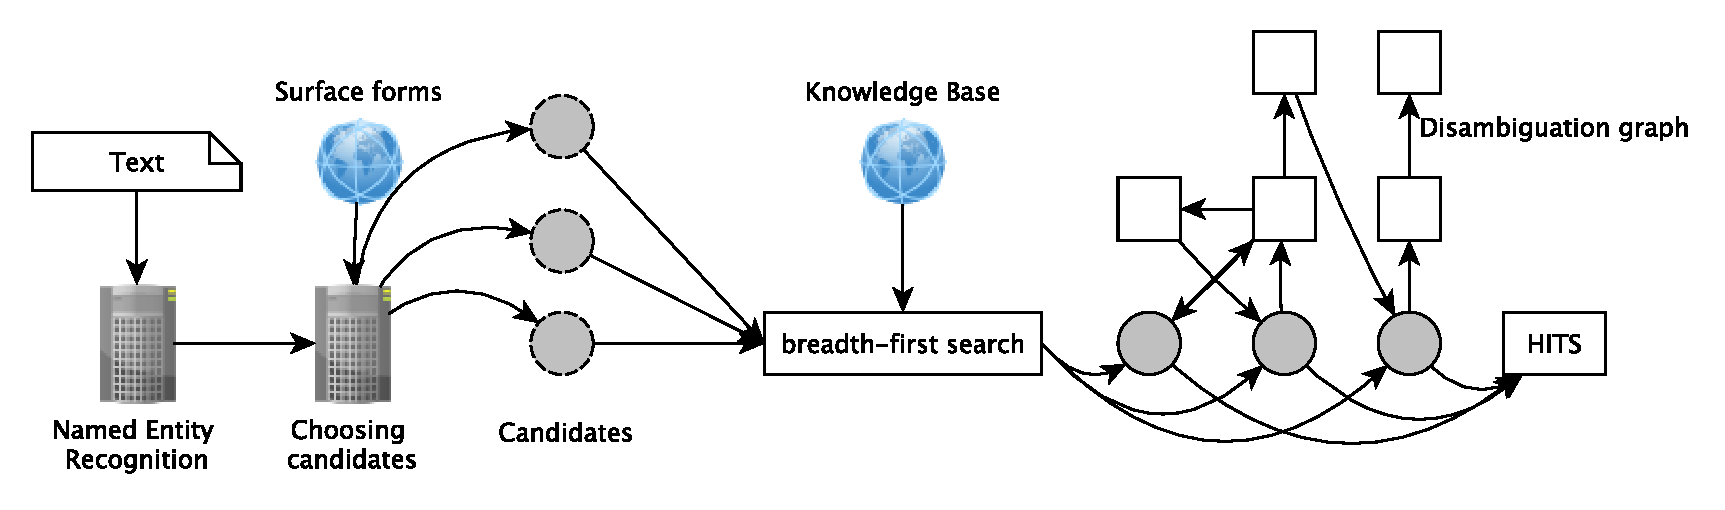
\includegraphics[width=\linewidth]{chapter_three/unstructured_annotation/fig/overview.pdf}
\caption{Overview of AGDISTIS.}
\label{fig:overview_agdistis}
\end{figure*}
%\todo[inline]{caption bei Änderung des Titels anpassen}

Our approach to NED thus consists of three main phases as depicted in Figure~\ref{fig:overview_agdistis}.
Given an input text $T$ and a named entity recognition function (e.g., FOX~\cite{FOX}), we begin by retrieving all named entities from the input text.
Thereafter, we aim to detect candidates for each of the detected named entities.
To this end, we apply several heuristics and make use of known surface forms~\cite{spotlight} for resources from the underlying KB.
The set of candidates generated by the first step is used to generate a disambiguation graph. 
Here, we rely on a graph search algorithm which retrieves context information from the underlying KB. 
Finally, we employ the HITS algorithm to the context graph to find authoritative candidates for the discovered named entities.
We assume that the resources with the highest authority values represent the correct candidates.
All algorithms in AGDISTIS have a polynomial time complexity, leading to AGDISTIS also being polynomial in time complexity.
Choosing candidates relates to the notion of $\phi$ while calculating the authority values confers to $\psi$.
In the following, we present each of the steps of AGDISTIS in more detail.

\subsection{Candidate Detection}\label{choosing}

In order to find the correct disambiguation for a certain set of named entities, we first need to detect candidate resources in the KB. 
We begin by creating an index comprising all labels of each resource.
Our approach can be configured to use any set of properties as labeling properties (e.g., those in Ell et al.~\cite{ELL+11}). 
For our experiments, we only considered \texttt{rdfs:label} as labeling property.
In addition, our approach can make use of known \emph{surface forms} for each of the resources in case such knowledge is available~\cite{spotlight}.
These are simply strings that are used on the Web to refer to given resources.
Surface forms are simply added to the set of available labels for each resource, cf.\ Section~\ref{eval}.
In this paper, we do not consider abbreviations although these could be easily regarded by adding further labels into the KB (e.g., via WordNet\footnote{\url{http://wordnet.princeton.edu/}}).
%\todo[inline]{remove the above sentence because of missing scientific eval?}

Next to searching the index we apply a \emph{string normalization} approach and an \emph{expansion policy} to the input text:
The string normalization is based on eliminating plural and genitive forms, removing common affixes such as postfixes for enterprise labels and ignoring candidates with time information (years, dates, etc.) within their label.
For example, the genitive \texttt{New York's} is transformed into \texttt{New York}, the postfix of \texttt{Microsoft Ltd.} is reduced to \texttt{Microsoft} and the time information of \texttt{London 2013} is ignored.
Our \emph{expansion policy} is a time-efficient approach to coreference resolution, which plays a central role when dealing with text from the Web, cf.~Singh et al.~~\cite{Singh}. 
In web and news documents, named entities are commonly mentioned in their full length the first time they appear, while the subsequent mentions only consist of a substring of the original mention due to the brevity of most news data.
For example, a text mentioning Barack Obama's arrival in Washington D.C. will commonly contain \texttt{Barack Obama} in the first mention of the entity and use strings such as \texttt{Obama} or \texttt{Barack} later in the same text (see Example~\ref{ex:obama}).
We implement this insight by mapping each named entity label (e.g., \texttt{Obama}) which is a substring of another named entity label that was recognized previously (e.g., \texttt{Barack Obama}) to the same resource ,\,i.e., \texttt{dbr:Barack\_Obama}.
If there are several possible expansions, we choose the shortest as a fast coreference resolution heuristic for web documents.
Without the expansion policy AGDISTIS suffers from a loss of accuracy of $\approx4\%$.

%This is simply due to humans readers being able to carry out a co-reference analysis on the fly.

%Internally, AGDISTIS begins its disambiguation by employing the string expansion policy\footnoterecall{myfootnote}.
%Our policy stores all named entity strings in order of their string length.
%If we recognize an entity string matching a part of an already processed entity, we expand the current string to the one stored earlier.
%This assumes both named entities mention the same instance.


%After expanding named entities we harness additional well-known linguistic heuristics.
%Named entities occur often in plural and genitive forms,\,i.e., AGDISTIS tries to identify and stem those words. 
%For example, the genitive form of the named entity \texttt{Obama's} is transformed into \texttt{Obama}.
%Additionally, AGDISTIS reduces plural strings such as \texttt{Obamas} to the singular form \texttt{Obama}.
%Another heuristic is to remove common affixes. 
%For example, we remove affixes which stands for the form of enterprises, such as \emph{corp} and \emph{ltd},\,e.g., \texttt{Hanover Insurance Corp.} is shrunk to \texttt{Hanover Insurance} in order to find candidates for this string in the KB.  	
%We observed a significant data quality problem considering affixes in the examined knowledge bases.
%AGDISTIS also eliminates candidates with years and dates within the label so as to be time-independent and to prune the search space.
%One key advantage of Linked Data is the possibility to retrieve a class for each instance in a KB.
%By using entity types (obtained via the \texttt{rdf:type} property), a domain fitting of possible candidates is implemented, narrowing the search space. 
Additionally, AGDISTIS can be configured to fit named entities to certain domains to narrow the search space.
Since our goal is to disambiguate persons, organizations and places, AGDISTIS only allows candidates of the types mentioned in Table~\ref{tab:tableOfClasses} when run on DBpedia and YAGO2.
Adding general types will increase the number of candidates and thus decrease the performance.
Obviously, these classes can be altered by the user as required to fit his purposes. 

\begin{table*}[htb!]
\centering
 \caption{DBpedia  and YAGO2 classes used for disambiguation classes. Prefix \texttt{dbo} stands for \texttt{http://dbpedia.org/ontology/}, \texttt{foaf} for \texttt{http://xmlns.com/foaf/0.1/} and \texttt{yago} for \texttt{http://yago-knowledge.org/resource/}.}
 \begin{tabular}{lll}
	\toprule
\textbf{} & \textbf{Class} & \texttt{\textbf{rdf:type}}\\
\midrule
DBpedia & Person & dbo:Person, foaf:Person\\
DBpedia & Organization & dbo:Organization, dbo:WrittenWork (e.g., Journals) \\
DBpedia & Place & dbo:Place, yago:YagoGeoEntity \\
\midrule
YAGO2 & Person & yago:yagoLegalActor  \\
YAGO2 & Organization & yago:yagoLegalActor, \\
  &   &  yago:wordnet\_exchange\_111409538 (e.g., NASDAQ) \\
YAGO2 & Place & yago:YagoGeoEntity \\
\bottomrule
\label{tab:tableOfClasses}
 \end{tabular}
 \end{table*}

\begin{algorithm}[htb!]
\KwData{label of a certain named entity $N_i$, $\sigma$ trigram similarity threshold}
\KwResult{$C$ candidates found}
$C \longleftarrow \emptyset$\;
{\bf label } $\longleftarrow$ {\bf normalize(label)}\;
{\bf label } $\longleftarrow$ {\bf expand(label)}\;
$ \displaystyle \bar C \longleftarrow$ {\bf searchIndex(label)}\;
\For{{\bf c} $\in \bar C$}{
    \If{$\neg${\bf c .matches([0-9]$^+$)}}{
        %\If{$\neg${\bf isDisambiguationSite(c})} {
         %          {\bf continue}\;
          %      }
        \If{{\bf trigramSimilarity(c, label)}$ \geq \sigma$}{
            \If{{\bf fitDomain(c)}} {
                $C \longleftarrow C \cup $ {\bf c}\;
            }
        }
        % The same as the two ifs above but with a continue
        %\If{{\bf trigramSimilarity(c, label)}$ < \sigma$} {
        %           {\bf continue}\;
        %        }
        %% {\bf c} $\longleftarrow$ {\bf redirect(c)}\;
        %\If{{\bf fitDomain(c)}} {
        %     $C \longleftarrow C \cup $ {\bf c}\;
        %        } 
        %}
    }
}
\caption{Searching candidates for a label.}
\label{findingCandidates}
\end{algorithm}

The resulting candidate detection approach is explicated in Algorithm~\ref{findingCandidates}.
%If a KB provides redirect and disambiguation URLs, AGDISTIS can benefit from them.
%\todo[inline]{added  a virtual function in this algorithm 1 for the grammatical functions}
%For example, it is straightforward to use \texttt{dbo:wikiPageRedirects} for identifying multiple labels for one instance. 
%Of course AGDISTIS ignores disambiguation entities as they would not help accomplishing the disambiguation goal and finding $\mu^{+}$. 
%\todo[inline]{AN:What's a disambiguation entity?}
In its final step, our system compares the heuristically obtained label with the label extracted from the KB by using \emph{trigram similarity} which is an n-gram similarity with $n=3$. 


\subsection{Computation of Optimal Assignment}

Given a set of candidate nodes, we begin the computation of the optimal assignment by constructing a disambiguation graph $G_d$ with search depth $d$.
To this end, we regard the input knowledge base as a directed graph $G_K = (V, E)$ where the vertices $V$ are resources of $K$, the edges $E$ are properties of $K$ and $x,y\in V, (x,y) \in E \Leftrightarrow \exists p : (x, p, y) \mbox{ is an RDF triple in }K$.
Given the set of candidates $C$, we begin by building an initial graph $G_0 = (V_0, E_0)$ where $V_0$ is the set of all resources in $C$ and $E_0=\emptyset$. %$\forall (x, y) \in V_0^2, (x, y) \in E_0 \Rightarrow (x, y) \in K$.
Starting with $G_0$ we extend the graph in a breadth-first search manner.
Therefore, we define the extension of a graph $G_i = (V_i, E_i)$ to a graph $\rho(G_i) = G_{i+1} = (V_{i+1}, E_{i+1})$ with $i=0, \ldots, d$ as follows:
\begin{equation}
V_{i+1} = V_i \cup \{y : \exists x \in V_i \wedge (x, y) \in E\}
\end{equation}
\begin{equation}
E_{i+1} = \{(x,y) \in E: x, y \in V_{i+1}\}
\end{equation}
We iterate the $\rho$ operator $d$ times on the input graph $G_0$ to compute the initial disambiguation graph $G_d$.

%Empirically, we see no effect on the \mbox{F-measure} when using spread activation instead~\cite{Kleb11WIMS} (despite the obvious extra computational costs).

After constructing the disambiguation graph $G_d$ we need to identify the correct candidate node for a given named entity.
Using the graph-based HITS algorithm we calculate authoritative values $x_a,y_a$ and hub values $x_h,y_h$ for all $x,y\in V_d$.
We initialize the authoritative and hub values (3) and afterwards iterate the equations (4) $k$ times as follows: 
\begin{align*}
\forall x \in V_d, x_a=x_h=\frac{1}{|V_d|} &\text{ (3) and } 
x_a\longleftarrow  \sum_{(y,x)\in E_d} y_h, \quad
y_h\longleftarrow \sum_{(y,x)\in E_d} x_a \text{(4)}
\end{align*}
We choose $k$ according to Kleinberg~\cite{HITS},\,i.e., 20 iterations, which suffice to achieve convergence in general. %d authoritative values $x_a$ and hub values $y_h$.
Afterwards we identify the most authoritative candidate $C_{ij}$ among the set of candidates $C_i$ as correct disambiguation for a given named entity $N_i$. %sort the nodes according to their authoritative values in descending order. 
%The first candidate for a certain named entity is assumed to be the correct disambiguation.
When using DBpedia as KB and $C_{ij}$ is a redirect AGDISTIS uses the target resource. %follows redirecting resources transitively. %can use redirections to di%maps redirecting resources to their most authoritative redirection.
AGDISTIS' whole procedure is presented in Algorithm~\ref{algooverview}.
As can be seen, we calculate $\mu^{+}$ solely by using polynomial time complex algorithms.
%Thus, we observe on average better run time performance than the state-of-the-art approach AIDA, see Section~\ref{results}. % Appendix Figure 3).
%\todo[inline]{Again, we have no Appendix here}
\begin{algorithm}
\KwData{$N=\{N_1,N_2\dots N_n\}$ named entities, $\sigma$ trigram similarity threshold, $d$ depth, $k$ number of iterations}
\KwResult{$C = \{C_1,C_2\dots C_n\}$ identified candidates for named entities}
$E \longleftarrow \emptyset$\;
$V \longleftarrow${\bf insertCandidates($N, \sigma$)}\;
$G \longleftarrow (V,E)$\;
$G \longleftarrow${\bf breadthFirstSearch($G,d$)}\;
{\bf HITS($G(V,E), k$)}\;
{\bf sortAccordingToAuthorityValue(V)}\;
\For{$N_i \in N$} {
    \For{$v \in V$}{
        \If{$v$ {\bf is a candidate for} $N_i$  }{
              {\bf store($N_i$,$v$)}\;
              {\bf break}\;
          }
     }
}
\caption{Disambiguation Algorithm based on HITS and Linked Data.}\label{algooverview}
\end{algorithm}

For our example, the graph depicted in Figure~\ref{fig:example} shows an excerpt of the input graph for the HITS disambiguation algorithm when relying on DBpedia as knowledge base. 
%Depending on the used KB properties may exist that lead to bi-directional edges (e.g., \texttt{sex} vs. \texttt{fatherOf}).
The results can be seen in Table~\ref{tab:example}. 
%Obviously a disambiguation towards the correct named entity URIs is possible.
%\todo{what happens if the KB does not contain the correct entity, does the algorithm answer null, but is encompanied with closed world assumption, we know all entities we annotated}
%Since we assume a closed-world scenario our algorithm supposes every entity to be in the KB.

\begin{figure}[htbp]
	\begin{minipage}[b]{0.57\textwidth} 
       % \begin{figure}
         \centering
        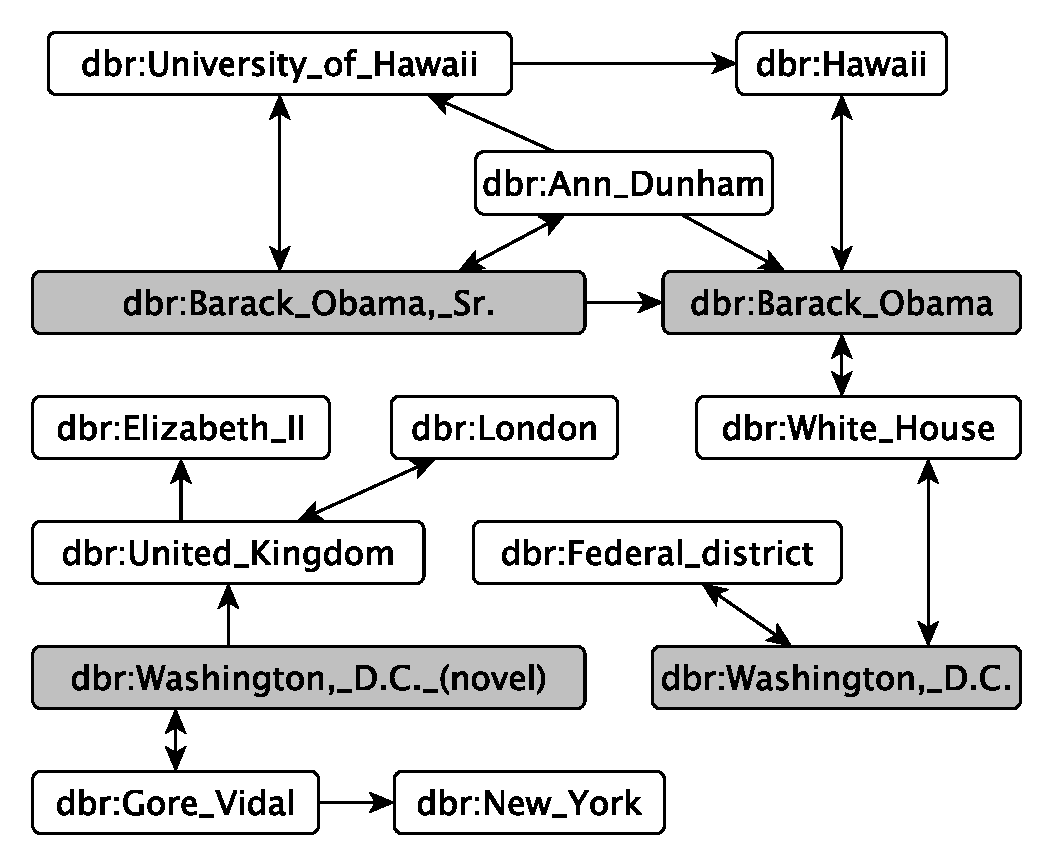
\includegraphics[width=\linewidth]{chapter_three/unstructured_annotation/fig/exampleGraph.pdf}
        \caption{One possible graph for the example sentence, with candidate nodes in grey.}
        \label{fig:example}
      %  \end{figure}
    \end{minipage}
	\hfill
	\begin{minipage}[b]{0.42\textwidth}
       % \begin{table}
        \centering
        \begin{tabular}{lc}
            \toprule
            \textbf{Node}  & \textbf{$x_a$} \\
            \midrule
            db:Barack\_Obama & 0.273 \\
            db:Barack\_Obama,\_Sr. & 0.089 \\
            db:Washington,\_D.C. & 0.093 \\
            db:Washington,\_D.C.\_(novel) & 0.000 \\
            \bottomrule
        \end{tabular}
        \captionof{table}{Authority weights for example graph.}
        \label{tab:example}
        \vspace{1.8cm}
       % \end{table}
	\end{minipage}
\end{figure}

%%Idea of the extension
%The most words of a document given to AGDISTIS are no named entities.
%Therefore, AGDISTIS does not use them in its workflow.
%Because a human reader would use all words for the disambiguation task we thought of an extension of AGDISTIS which uses the additional words, too.
%With these words AGDISTIS would be able to recognize the topical structure of the document and could use these information for the disambiguation task.
%Therefore, we added an extension which uses topic modeling to consider the topical structure.

%%what is topic modeling
%\emph{Probabilistic topic modeling} is a research area that aims to discover thematic information inside large corpora \cite{Blei:2012:PTM:2133806.2133826}.
%It is based on the definition of generative models that describe the creation of documents and how this process is influenced by latent topics.
%A very famous model is \emph{Latent Dirichlet Allocation (LDA)} \cite{Blei:2003:LDA:944919.944937}.
%Its generative process is based on a set of Topics $T$ and a vocabulary $V$.
%For the creation of a document $d$ the distribution of the topics inside this document $\theta_d=\left \{P(t_0|d), \ldots, P(t_{|T|}|d) \right \}$ is sampled.
%After that for every $i$th-word the id $z_i$ of a topic $t_{z_i}$ is sampled from $\theta_d$.
%Every topic $t \in T$ has a vector $\phi_{t}=\left \{P(w_0|t), \ldots, P(w_{|V|}|t) \right \}$ which defines the probabilities of all words under this topic.
%After $z_i$ has been sampled the word is sampled from $\phi_{t_{z_i}}$ \cite{Blei:2012:PTM:2133806.2133826}.
%Figure TODO shows the graphical model of LDA.
%The figure contains $\alpha$ and $\beta$ which are hyperparameter for the $\theta$ and $\phi$ distributions respectively.
%\todo[inline]{Add graphic with plate notation}

%In figure TODO all variables are white except the word $w$ which is shaded.
%This means that $w$ is the only variable which can be observed and all other variables are latent.
%So starting with the observable words inside of the documents of a corpus the other variables have to be inferenced.
%Because a direct solution of the inference problem is intractable there are several algorithms for approximating the variables \cite{Blei:2012:PTM:2133806.2133826}.
%For our experiments we used Mallet which contains an implementation of Gibbs-Sampling \cite{McCallumMALLET,griffiths2004finding}.

%\todo[inline]{* definition \newline* LDA \newline* generative model \newline* how do we use it \newline* where does the model come from\newline * \textbf{what are we doing with the model and the texts}}

\section{Evaluation}
\label{sec:eval}

\subsection{Experimental Setup}
\label{eval}
The aim of our evaluation was two-fold.
First, we wanted  to determine the F-measure achieved by our approach on different datasets.
Several definitions of F-measure have been used in previous work on NED.
Cornolti et al.~\cite{cornolti} define the micro F-measure (F1) w.r.t. a strong annotation match (i.e., a binary relation) and the possibility of assigning null to an entity.
This F-measure, which we use throughout our evaluation, aggregates all true/false positives/negatives over all documents.
Thus, it accounts for larger contexts in documents with more annotations, cf. Cornolti et al.~\cite{cornolti}.

%In addition to the traditional definition of false and true positives and negatives when given a reference mapping between strings and resources, 
%we regarded the assignment of a resource to a string as a \emph{false positive} if no resource from the KB mapped with the string or if the string was assigned to the wrong resource.
%Furthermore, the assignment of a resource was considered a \emph{false negative} if the approach returned that no resource mapped the string although there was a resource in the KB that did.

Second, we wanted to know how AGDISTIS performs in comparison to other state-of-the-art NED approaches. 
Thus, we compare AGDISTIS with TagMe 2, the best approach according to ~\cite{cornolti} as well as with AIDA and DBpedia Spotlight because they are well-known in the Linked Data community. 
AGDISTIS is designed to be agnostic of the underlying knowledge base.
Thus, we use the German and English DBpedia KB as well as the English YAGO 2 KB. %\footnote{Results using other Linked Data KBs can be found at the project homepage.}

Within our experiments, we ran AGDISTIS with the following parameter settings: 
the threshold $\sigma$ for the trigram similarity was varied between 0 and 1 in steps of 0.01. 
Additionally, we evaluated our approach with $d=1,2,3$ to measure the influence of the size of the disambiguation graph on AGDISTIS' F-measure.
%In this paper we use accuracy to measure directly the percentage of correctly disambiguated entities instead of the also common precision and recall values.
%We also ran the experiments without using the graph,\,i.e., only applying all heuristics and trigram similarity.
%We did not consider abbreviations and thus ignored labels shorter than three characters.
For our experiments, we fitted AGDISTIS to the domain of named entity recognition and only allow candidates of the types mentioned in Table~\ref{tab:tableOfClasses}.
%While, we were not able to identify all entities in all datasets resulting in a worse F1-measure than possible. 
%Moreover, %a closed world was assumed,\,i.e., entities that were not in the KB were not considered in our evaluation.
%We used YAGO2 (English) as well as the German and the English versions of DBpedia as underlying KBs for AGDISTIS.
%While the results reported in this paper only use the English versions of DBpedia 3.9 as underlying KB, we also evaluated AGDISTIS on YAGO2 and the German version of DBpedia 389. 
We report more details on the evaluation setup as well as complete results at the project homepage.
%\todo[inline]{Micha: But this would be possible now, wouldn't it?}

%Note that for most entities from DBpedia a direct matching to YAGO2 entities can easily be applied. 
%Web news texts are a common input for disambiguation systems~\cite{Cucerzan07,fox}.
%Third, we wanted to measure how time-efficient AGDISTIS is. 
%To this end, we compared its runtime with that of AIDA.
%We were not able to compare AGDISTIS' runtime with that of Spotlight due to Spotlight's high RAM requirements.
%\todo[inline]{not RAM but webservice}
%Finally, we analyzed the impact of removing certain properties on the \mbox{F-measure}.
%We carried out all our experiments on the following four datasets:\newline
%: (1) a subset of the well-known Reuters-21578 dataset, (2) RSS feeds extracted from 1,500 sources, (3) a German news corpus extracted from \url{news.de} and (4) the original AIDA dataset from~\cite{AIDA}, which contains 1,393 annotated news reports.
%%For each corpus, we generated a spell-corrected version of annotations. % assuming that a used disambiguation system would incorporate such a module.
%%\todo[inline]{Discuss whether pointing to a spell corrected version can be left out}
%We annotated the first dataset manually while the others were already annotated and used in previous works.
%%Some documents comprise only little or no annotations to account for the sparsity and shortness of WND. 
%%Furthermore, only the in Table~\ref{tab:tableOfClasses} mentioned resource classes were annotated.
%%\todo{explain why reagan and not reagan area is annotated}
%\footnote{To preserve the anonimity of the authors, we refrained from adding a link to the page for downloading the data. A link to this page will be added in the final version of the paper.}
%The test corpora can be downloaded from \url{https://github.com/XYZ}.%https://github.com/AKSW/AGDISTIS}.

\subsection{Datasets}
Noisy and incorrect datasets can affect the performance of NED approaches which can be prevented by using well-known datasets.
We carried out our evaluation on the following eight different, publicly available datasets, which consists of the three corpora from the benchmark dataset \textbf{N3}~\cite{n3}, the original AIDA evaluation corpus\footnote{\url{https://www.mpi-inf.mpg.de/departments/databases-and-information-systems/research/yago-naga/aida/downloads/}} and four of the five datasets from the Cornolti et al.~\cite{cornolti} benchmark:

\begin{enumerate}
\item \textbf{Reuters-21578 Dataset.}
The first of the N3 datasets comprises 145 news articles randomly sampled from the Reuters-21578 news articles dataset.
Two domain experts determined the correct URI for each named entity using an online annotation tool reaching a initial voter agreement of $74\%$.
%Although we have no agreement values for AIDA, we consider 74\% as an upper bound for human capability for NED tasks.
%In comparison, DBpedia Spotlight achieved a \emph{Fleiss' Kappa} maximum of 0.67~\cite{spotlight} during creation of their dataset.
%\todo{compare the interrater agreement with the one of AIDA: AIDA didn't mention agreement rate, AIDA used 2 students and resolved in case of conflict}
In cases where the judges did not agree initially, they concerted each other and reached an agreement.
This initial agreement rate hints towards the difficulty of the disambiguation task.
The corpus does not annotate ticker symbols of companies (e.g., \textit{GOOG} for Google Inc.), abbreviations and job descriptions because those are always preceded by the full company name respectively a person's name.
%Since AGDISTIS relies on a closed-world assumption, 
%Finally, we generated a default URI for instances which could not be identified within a 5-minute Web search while annotating. 

\item \textbf{\url{news.de} Dataset.}
This real-world dataset is the second of the N3 datasets and was collected from 2009 to 2011 from the German web news portal \url{news.de} ensuring that each message contains the German word \emph{Golf}.
This word is a homonym that can semantically mean a geographical gulf, a car model or the sport discipline.
This dataset contains 53 texts comprising over 600 named entities that were annotated manually by a domain expert.
Although some meanings of Golf are not within the class range of our evaluation, they are kept for evaluation purposes.

\item \textbf{RSS-500 Dataset.}
This corpus has been published in Gerber et al.~\cite{GER+13} and is the third of the of the N3 datasets.
It consists of data scrapped from 1,457 RSS feeds. % as compiled in Goldhahn~\shortcite{GOLDHAHN12.327}.
The list includes all major worldwide newspapers and a wide range of topics,\,e.g., \emph{World}, \emph{U.S.}, \emph{Business}, \emph{Science} etc.
This list was crawled for 76 hours, which resulted in a corpus of about 11.7 million sentences.
A subset of this corpus has been created by randomly selecting $1\%$ of the contained sentences.
Finally, domain experts annotated 500 sentences manually. 
Further information about the corpora and the datasets themselves can be found on the project homepage.\footnote{\url{http://aksw.org/Projects/N3NERNEDNIF.html}}
%These sentences were a subset of those which contained a natural language representation of a formal relation, like ``\ldots, who was born in\ldots '' for \texttt{dpo:birthPlace} (see ~\cite{conf/ekaw/GerberN12}), that occurred more then 5 times in the 1\% corpus. %with DBpedia URIs or created new URIs in case the mentioned entity was not contained in DBpedia.

\item \textbf{AIDA-YAGO2 Dataset.}
This is the original dataset that was used while evaluating AIDA~\cite{AIDA}, stemming from the CoNLL 2003 shared task~\cite{conll2003} and comprising 1,393 news articles which were annotated manually. % with 34,956 entity mentions.
%Possible conflicts resulting from two annotators were resolved.
%AIDA-YAGO2 has 34,956 entity mentions from the YAGO2 ontology.%\footnote{\url{http://www.mpi-inf.mpg.de/yago-naga/yago/}}.

\item  \textbf{AIDA/CO-NLL-TestB} This dataset (like all the subsequent datasets) comes from the Cornolti et al. benchmarks and originates from the evaluation of AIDA~\cite{AIDA}. 
As mentioned above, this dataset was derived from the CO-NLL 2003 shared task~\cite{conll2003} and comprises 1,393 news articles which were annotated manually. Two students annotated each entity resolving conflicts by the authors of AIDA~\cite{AIDA}. Cornolti et al.'s benchmark consists only of the second test part comprising 231 documents with 19.4 entities per document on average.

\item \textbf{AQUAINT} In this dataset, only the first mention of an entity is annotated. The corpus consists of 50 documents which are on average longer than the AIDA/CO-NLL-TestB documents. Each document contains 14.5 annotated elements on average
The documents originate from different news services, e.g. Associated Press and have been annotated using voter agreement.
The dataset was created by Milne et al.~\cite{milne2008learning}.

\item \textbf{IITB} The IITB corpus comprises 103 manually annotated documents. Each document contains 109.1 entities on average.
This dataset displays the highest entity/document-density of all corpora.
This corpus has been presented by Kulkarni et al.~\cite{kulkarni2009collective} in 2009.

\item \textbf{MSNBC} This corpus contains 20 news documents with 32.9 entities per document. This corpus was presented in 2007 by Cucerzan et al.~\cite{Cucerzan07}.
\end{enumerate}

We did not use the \textbf{Meij} dataset from Cornolti et al. since it comprises only tweets from twitter with 1.6 entities per document. The number of entities available in the datasets is shown in Table~\ref{tab:data}.
%\todo{leave the computer stuff out?}
All experiments were carried out on a MacBook Pro with a 2.7GHz Intel Core i7 processor and 4 GB 1333MHz DDR3 RAM using Mac OS 10.7. 
\begin{table*}[tb!]
\centering
\caption{Test corpora specification including the number of documents (\#Doc.) and the number of named entities (\#Ent.) per dataset}
\label{tab:data}
\begin{tabular}{lcrrrc}
\toprule
\textbf{Corpus} & \textbf{Language} & \textbf{\#Doc.} & \textbf{\#Ent.} & \textbf{Ent./Doc.} & \textbf{Annotation}\\
\midrule
AIDA/CO-NLL-TestB  & English & 231 & 4458 &19.40& voter agreement\\
AQUAINT & English & 50 & 727 & 14.50 &voter agreement\\
IITB & English & 103 & 11,245 & 109.01 &domain expert\\
MSNBC & English & 20 & 658 &31.90 &domain expert\\
Reuters-21578  & English & 145 & 769 &5.30 &voter agreement\\
RSS 500 & English & 500 & 1,000 & 2.00&domain expert \\
\url{news.de} & German & 53 & 627 & 11.83 &domain expert\\
AIDA-YAGO2 & English & 1,393 & 34,956 &25.07 &voter agreement\\
\bottomrule
\end{tabular}
\end{table*}

%\begin{figure*}[tb!]
%    \centering
%        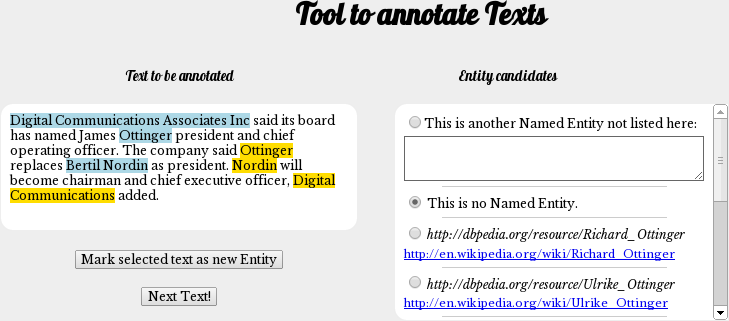
\includegraphics[width=\linewidth]{fig/qrtoolnew.png}
%    \caption{GUI of our annotation tool.}
%    \label{fig:qrtool}
%\end{figure*}

\subsection{Results}
\label{results}

\begin{table*}[hb!]
\centering
\caption{Evaluation of AGDISTIS against AIDA and DBpedia Spotlight. Bold indicates best \mbox{F-measure}.} \label{tab:evalold} 
\begin{tabular}{c ccc ccc c c}
\toprule
\textbf{Corpus}  & \multicolumn{6}{c}{\textbf{AGDISTIS}}	& \textbf{AIDA} & \textbf{Spotlight}\\\midrule
\textbf{$K$}& \multicolumn{3}{c}{{DBpedia}}& \multicolumn{3}{c}{{YAGO2}}	& {YAGO2} & {DBpedia}\\\midrule
				& \mbox{F-measure} 		& $\quad \sigma \quad $ & $\quad d \quad $ 	& \mbox{F-measure} & $\quad \sigma \quad $ & $\quad d \quad $ & \mbox{F-measure}  & \mbox{F-measure}\\
\cmidrule(r){2-4}  \cmidrule(r){5-7} \cmidrule{8-8} \cmidrule{9-9}
Reuters-21578	&  	\textbf{0.78}	&  			0.87		&  		2		& 	0.60	&  0.29		&  	3	&  	0.62		& 	0.56	\\
RSS-500 		&  	\textbf{0.75}	&  			0.76		&  		2		& 	0.53	&  0.82		&   2 	&  	0.60		& 	0.56	\\
\url{news.de} 	&  	\textbf{0.87}	&  			0.71		&  		2		& 	---		&   ---		&  ----	&  	----		& 	0.84	\\
AIDA-YAGO2	   	&  		0.73		&  			0.89		&  		2		& 	0.58	&  0.76		&   2 	&\textbf{0.83}	& 	0.57	\\
\bottomrule
\end{tabular}
\end{table*}

First, we evaluate AGDISTIS against AIDA and DBpedia Spotlight on three different knowledge bases using N3 corpora and the AIDA-YAGO2 corpus. 

AGDISTIS performs best on the \url{news.de} corpus, achieving a maximal 0.87 \mbox{F-measure} for $\sigma = 0.71$ and $d = 2$ (see Table~\ref{tab:evalold}).
Our approach also outperforms the state of the art on Reuters-21578 corpus (see Figure~\ref{fig:reuters}), where it reaches 0.78 \mbox{F-measure} for $\sigma = 0.87$ and $d = 2$.
Considering the AIDA-YAGO2 dataset AGDISTIS achieves an \mbox{F-measure} of 0.73 for $\sigma = 0.89$ and $d = 2$.
%In combination with the results on RSS-500, 
Our results suggest that $d=2, \sigma=0.82$ and using DBpedia as KB are a good setting for AGDISTIS and suffice to perform well. %The iteration of $\sigma$ between $0.7$ and $0.9$ can lead to an improvement of up to $6\%$ \mbox{F-measure}.
In the only case where $\sigma=0.29$ leads to better results (Reuters-21578 corpus), the setting $0.7<\sigma<0.9$ is only outperformed by 0.03 F-measure using YAGO as KB for AGDISTIS.

\begin{table}
    \centering
\caption{Performance of AGDISTIS, DBpedia Spotlight and TagMe 2 on four different datasets using micro F-measure (\textbf{F1}).}
\begin{tabular}[tb]{@{}lllll@{}}
\toprule
Dataset                            & Approach          & \textbf{F1-measure}             & \textbf{Precision} & \textbf{Recall} \\ \midrule
\multirow{3}{*}{\begin{minipage}{0.8in}\textbf{AIDA/CO-NLL-TestB}\end{minipage}} & TagMe 2           & 0.565          & 0.58      & 0.551  \\
                                   & DBpedia Spotlight & 0.341          & 0.308     & 0.384  \\
                                   & AGDISTIS          & \textbf{0.596} & \textbf{0.642}     & \textbf{0.556}  \\ \midrule
\multirow{3}{*}{\textbf{AQUAINT}}  & TagMe 2           & 0.457          & 0.412     & \textbf{0.514}  \\
                                   & DBpedia Spotlight & 0.26           & 0.178     & 0.48   \\
                                   & AGDISTIS          & \textbf{0.547} & \textbf{0.777}     & 0.422  \\\midrule
\multirow{3}{*}{\textbf{IITB}}     & TagMe 2           & 0.408          & 0.416     & 0.4    \\
                                   & DBpedia Spotlight & \textbf{0.46}  & 0.434     & \textbf{0.489}  \\
                                   & AGDISTIS          & 0.31           & \textbf{0.646}     & 0.204  \\\midrule
\multirow{3}{*}{\textbf{MSNBC}}    & TagMe 2           & 0.466          & 0.431     & 0.508  \\
                                   & DBpedia Spotlight & 0.331          & 0.317     & 0.347  \\
                                   & AGDISTIS          & \textbf{0.761} & \textbf{0.796}     & \textbf{0.729}  \\ \bottomrule
\end{tabular}
\label{tab:evalnew}
\end{table}

Second, we compared our approach with TagMe 2 and DBpedia using the datasets already implemented in the framework of Cornolti et al.
AGDISTIS has been setup to use a breadth-first search depth $d=2$ and a trigram similarity of $\sigma=0.82$.
All approaches used disambiguate w.r.t. the English DBpedia.
%TagMe 2 and DBpedia Spotlight are easily to test via web services while AIDA needs to be installed locally and run on a large machine. 
AIDA was ommitted from this evaluation because it has been shown to be outperformed by TagMe 2 in~\cite{cornolti} on the datasets we consider. 

AGDISTIS achieves \mbox{F-measures} between $0.31$ (IITB) and $0.76$ (MSNBC) (see Table~\ref{tab:evalnew}).
We outperform the currently best disambiguation framework, TagMe 2, on three out of four datasets by up to $29.5\%$ F-measure. 
Our poor performance on IITB is due to AGDISTIS not yet implementing a paragraph-wise disambiguation policy. 
By now, AGDISTIS performs disambiguation on full documents.
The large number of resources in the IITB documents thus lead to our approach generating very large disambiguation graphs.
The explosion of errors within these graphs results in an overall poor disambiguation.
We will address this drawback in future work by fitting AGDISTIS with a preprocessor able to extract paragraphs from input texts.
The local vector-space model used by Spotlight performs best in this setting. 

%\todo[inline]{Micha: the part "The iteration of $\sigma$ between $0.7$ and $0.9$ can lead to an improvement of up to $6\%$ \mbox{F-measure}" occurs two times. Remove one of them.}  
\begin{figure}[htb!]\centering
        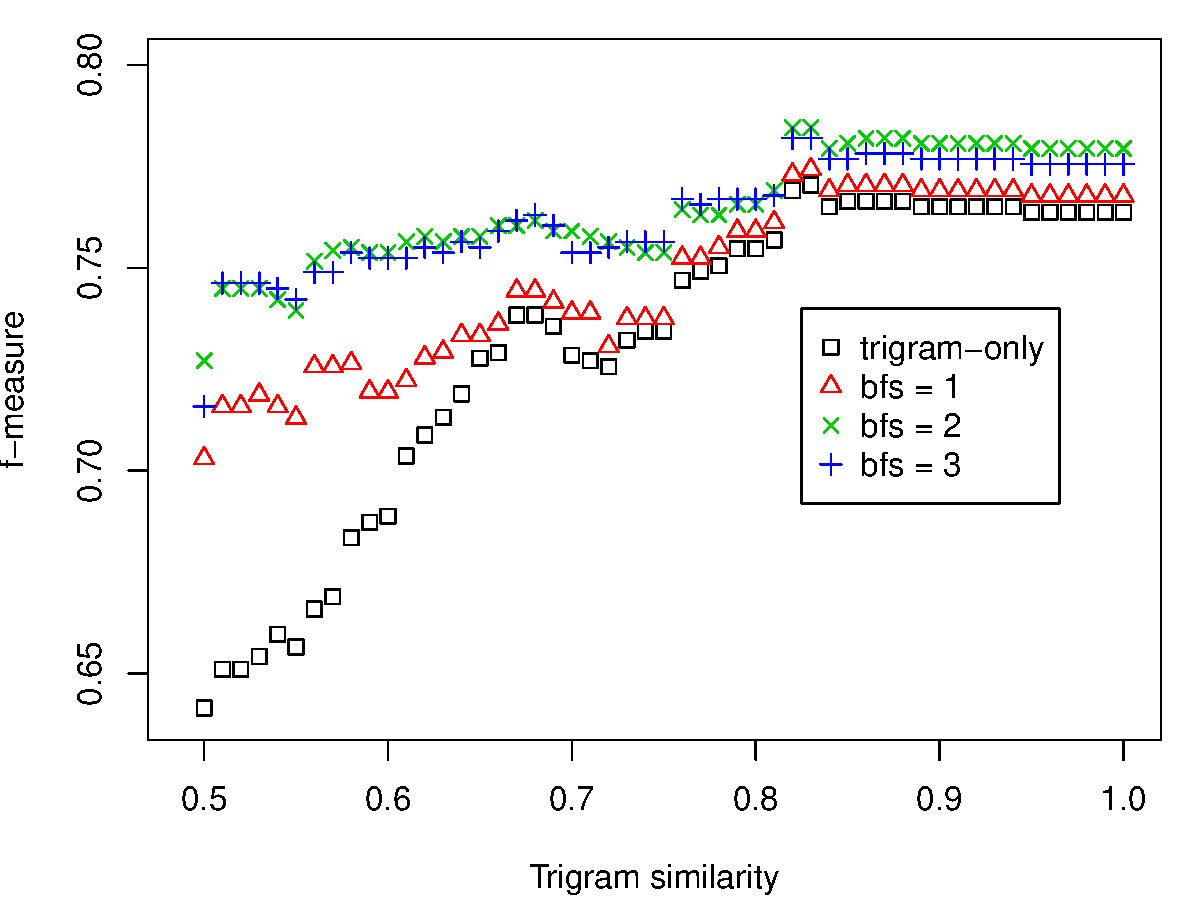
\includegraphics[width=0.9\linewidth]{chapter_three/unstructured_annotation/fig/reuters.pdf}
        %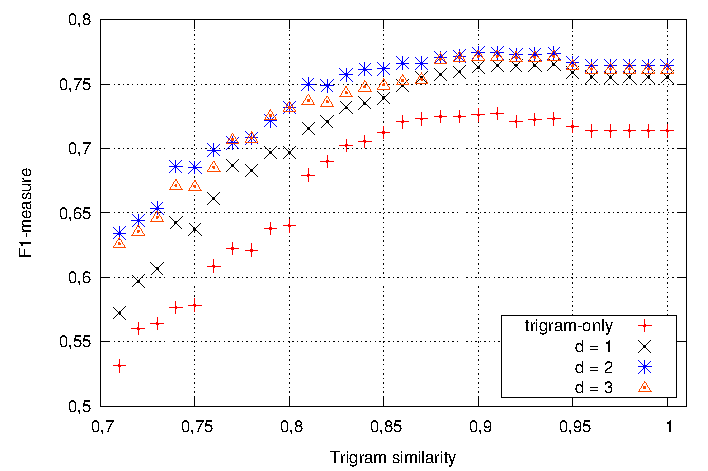
\includegraphics[width=0.9\linewidth]{fig/bfs_depth_diag.pdf}
    \caption{\mbox{F-measure} on the \textbf{Reuters-21578} corpus using DBpedia as KB.}  \label{fig:reuters}
\end{figure}

Delving deeper into AGDISTIS' results lead to the following insights:
(1) Varying the search depth $d$ does not significantly improve \mbox{F-measure} because within the underlying documents there are many similar named entities forming a shallow semantic background. However, using only string similarity measures ($d=0$) results in lower F-measure (see Figure \ref{fig:reuters}). % while the optimum has been found using $d=2$. %, see Figure~(\todo[inline]{here was a reference to a reuters figure}). 
(2) The expansion policy can have considerable knock-on effects: Either the first entity and its expansions are disambiguated correctly or the wrong disambiguation of the first entity leads to an avalanche of false results in a loss of $\approx 4\%$ accuracy.
%\todo[inline]{Micha: Why accuracy while you always talk about F-measure?}
(3) We observed a significant enhancement of AGDISTIS when adding surface forms to the labels of resources as explained in Section~\ref{choosing}.
Employing additional labels (such as surface forms gathered from Wikipedia) increased the \mbox{F-measure} of AGDISTIS by up to $4\%$. 
(5) Using $n=1,2,4$ as n-gram similarity has been proven to perform worse than using trigram similarity,\,i.e., $n=3$.
Our results suggest that $d=2$ while using DBpedia as KB is a good setting for AGDISTIS and suffice to perform well. 
The iteration of $\sigma$ between $0.7$ and $0.9$ can lead to an improvement of up to $6\%$ \mbox{F-measure} while $\sigma<0.7$ and $\sigma>0.9$ leads to a loss of F-measure.

Overall, our results suggest that $\sigma=0.82$ and $d=2$ is generally usable across datasets and knowledge bases leading to high quality results.\footnote{See also \url{http://139.18.2.164/rusbeck/agdistis/supplementary.pdf} and \url{http://139.18.2.164/rusbeck/agdistis/appendix.pdf}}
%Thus, in the following, we use $\sigma=0.82$. 

%This is done by selecting all resources as candidates that are such that the similarity of at least one of its labels and the 
%The best similarity thresholds $\sigma$ w.r.t. disambiguation \mbox{F-measure} achieved by our approach were determined empirically iterating $\sigma$ between 0 and 1 in steps of 0.01. 
%Setting $\sigma=0.82$ turned out to be the best threshold independent of the analysed dataset.%\footnote{See our project side for further evaluation \url{http://aksw.org/Projects/AGDISTIS}}% (cf. Section~\ref{eval}).
%as shown in Figure~\ref{fig:influenceOfSurfaceForms}.
%This explains the worse results achieved by AGDISTIS when using YAGO2 as KB. 

%\begin{figure}[htb!]\centering
%        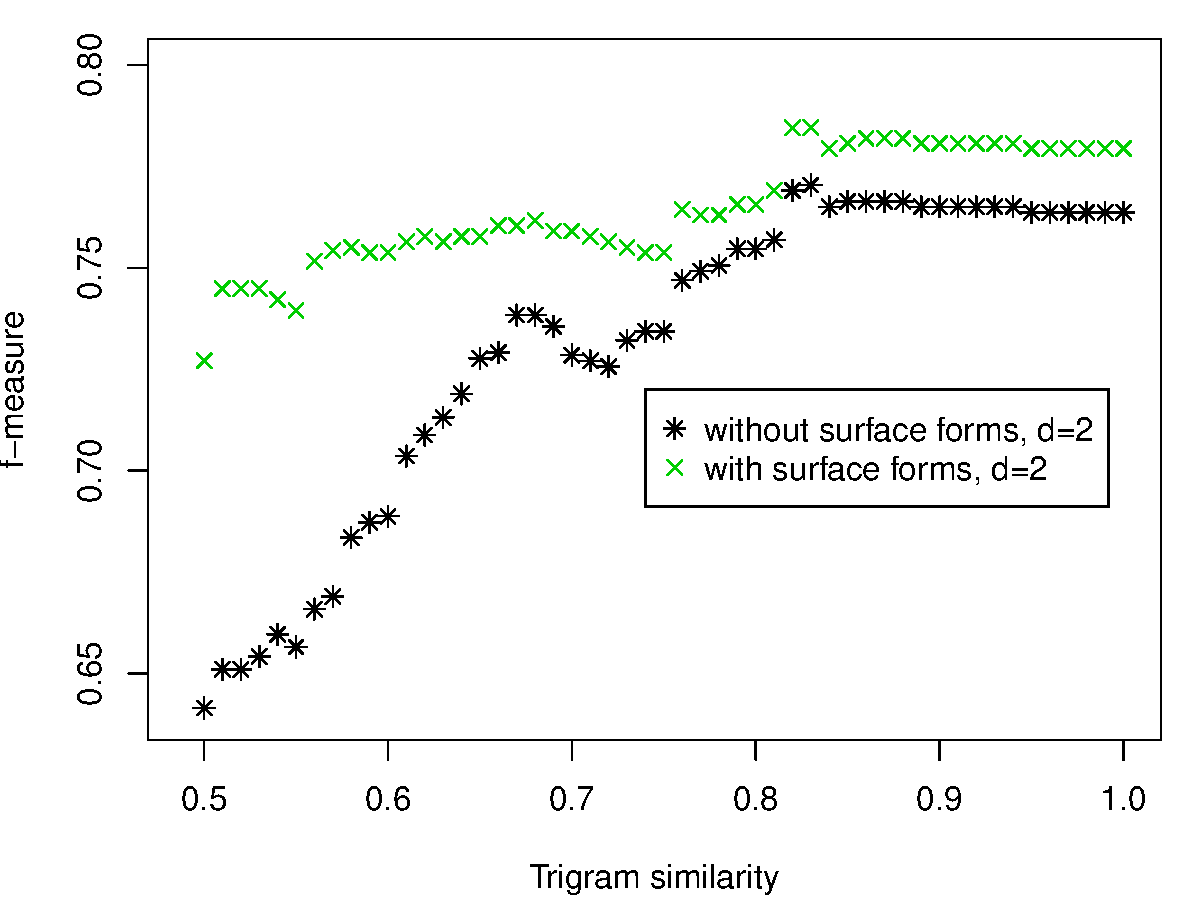
\includegraphics[width=0.9\linewidth]{fig/reutersWithoutSurfaceFormsAndBFS2.pdf}
        %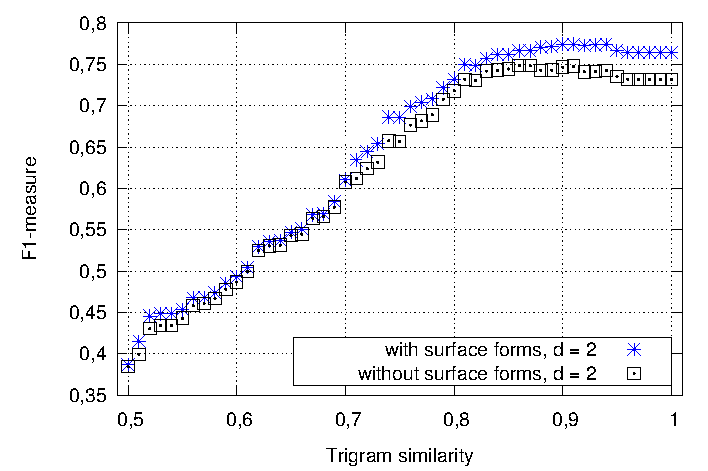
\includegraphics[width=0.9\linewidth]{fig/surface_forms_diag.pdf}
%    \caption{Influence of surface forms on the Reuters-21578 corpus and DBpedia as KB.}\label{fig:influenceOfSurfaceForms}
%\end{figure}
%\todo[inline]{@axel: not using any graph just trigram sim is worse than the rest}
% for AGDISTIS are worse since our approach could not make use of surface forms as explained above. %, redirects or disambiguation entities, as explained above.
%Yet, given that a 1-1 mapping exists between YAGO2 and DBpedia URIs, we will consider the results of DBpedia for AGDISTIS in the following comparisons with other tools.
%\todo[inline}]{AN:Formally wrong. Either a 1-1 mapping exists or it does not}
%If there is no 1-1 mapping, the result of the disambiguation is counted as \emph{false positive}, which then results in low \mbox{F-measures} using YAGO2 as KB.
%\todo{look at table caption please}


%\textbf{Comparison with AIDA.} 
%\todo[inline]{renew numbers}
%We compared our approach to AIDA by using the \textit{Cocktailparty configuration}\footnote{\url{https://github.com/yago-naga/aida}} (which is the recommended configuration for the framework) and applied the same restrictions that we used for AGDISTIS.
%The results of this evaluation on AIDA can be seen in Table~(\todo[inline]{here was a reference to the eval result}).
%Overall, AIDA performs well on arbitrary entities. 
%Yet, it is clearly outperformed by our approach on specific persons and organizations. 
%\todo[inline]{the statement above cant be seen in table 4, therefore we need to compare by type or clarify this sentence}
%In comparison to AIDA, AGDISTIS performs best on the Reuters-21578  where it surpasses AIDA by $\approx 0.16$ \mbox{F-measure}.
%Here AGDISTIS benefits from surface forms and its expansion policy.
%Furthermore, AGDISTIS outperforms AIDA with the RSS-500 corpus by $\approx 0.15$ \mbox{F-measure}.
%This corpus differs considerably from the Reuters-21578 corpus due to the small disambiguation contexts and graphs evolving from two named entities per text only.
%Note that AGDISTIS also outperforms AIDA for our overall default setting of $\sigma = 0.81$, apart from the result on the AIDA-YAGO2 corpus.
%AIDA could not be run on the \url{news.de} corpus as it can only deal with English.
%Here, the \emph{language-independence} of AGDISTIS provides a significant improvement of the state of the art.
%AIDA performs better on AIDA-YAGO2 achieving an \mbox{F-measure} of 0.83 due to the large contexts of the documents (see Table~(\todo[inline]{here was a reference to a data table})).
%This is clearly due to AGDISTIS being tuned towards smaller contexts since these are more common in WND, see Table~(\todo[inline]{here was a reference to a data table}).
%In particular, the AIDA-YAGO2 corpus contains many sport teams from cities and countries like \texttt{Barcelona} where AGDISTIS identifies \texttt{dbr:Barcelona} and \texttt{dbr:FC\_Barcelona} as resources. Since \texttt{dbr:Barcelona} has a higher authoritative score than \texttt{dbr:FC\_Barcelona}, AGDISTIS' disambiguation results in a \emph{false positive} in this particular case.
%As shown in Table~\ref{eval} using YAGO2 leads to worse results since AGDISTIS (in contrast to AIDA) does not possess surface forms for YAGO2.
%\todo[inline]{No appendiy, how to solve this?}

%\textbf{Comparison with DBpedia Spotlight.}
%\todo[inline]{renew the numbers}
%In order to compare DBpedia Spotlight with AGDISTIS Cornolti et al.~\cite{cornolti} used Spotlight's Web services.\footnote{\url{https://github.com/dbpedia-spotlight/dbpedia-spotlight/wiki/Web-service}}

%The results of the evaluation are shown in Table~\ref{tab:eval}.
%Spotlight performs best on the \url{news.de} dataset (\mbox{F-measure} = 0.84) and worst on the Reuters-21578 dataset (\mbox{F-measure} = 0.56), Table~(\todo[inline]{here was a reference to the eval result}).
%This is possibly due to the datasets age of over 20 years and missing historic data in DBpedia.
%When evaluated against the AIDA-YAGO2 corpus Spotlight achieves a \mbox{F-measure} of 0.57.
%Using the RSS-500 dataset Spotlight is only able to generate a \mbox{F-measure} of 0.56.
%\todo[inline]{renew the number}
%AGDISTIS outperforms Spotlight by at least $\approx 0.15$ \mbox{F-measure}. % using DBpedia as KB. on each English dataset.

%AGDISTIS performs better on two of the datasets and is even usable for the German dataset as it is agnostic towards the language of the used KB.
%As can be seen in Figure \ref{fig:relation} the number of entities per text is an important criteria for disambiguation.

%\textbf{Run time analysis.}
%On average AGDISTIS is more time-efficient than AIDA with respect to the best %corresponding configuration.
%While AGDISTIS finished its computation on Reuters-21578 corpus in 549\,seconds (s), AIDA needed more than twice as much time,\,i.e., 1,296\,s.
%This behavior can also be seen on the short documents of the RSS-500 dataset, where AIDA needed 4,919\,s and our approach only 623\,s.
%Moreover, AGDISTIS outperforms AIDA with 3,946\,s to 51,435\,s run time on the AIDA-YAGO2 corpus.
%\todo[inline]{is not comparable anymore since we needed to run it in the cloud}
%Details can be found on the project website.

\section{Conclusion}
\label{sec:conclusion}
%\todo[inline]{Micha: AIDA is missing in the conclusion.}
We presented AGDISTIS a novel named entity disambiguation that combines the scalable HITS algorithm and breadth-first search with linguistic heuristics.
Our approach outperforms the state-of-the-art algorithms TagMe 2, AIDA and DBpedia Spotlight while remaining quadratic in its time complexity. 
Moreover, our evaluation suggests that while the approach performs well in and of itself, it can benefit from being presented with more linguistic information such as surface forms. 
%Furthermore, we measured the effect of evolving the structure of the underlying knowledge base.
%We observed the significance of properties on the \mbox{F-measure} performance of our system.
%Our results suggest that only a few RDF properties contribute significantly to enhancing the performance of AGDISTIS.
We see this work as the first step in a larger research agenda.
Based on AGDISTIS, we aim to develop a new paradigm for realizing NLP services which employ community-generated, multilingual and evolving Linked Open Data background knowledge.
Other than most work, which mainly uses statistics and heuristics, we aim to truly exploit the graph structure and semantics of the background knowledge.

Since AGDISTIS is agnostic of the underlying knowledge base and language-independent, it can profit from growing KBs as well as multilingual Linked Data.
In the future, we will thus extend AGDISTIS by using different underlying KBs and even more domain-specific datasets.
An evaluation of Babelfy against our approach will be published on the project website.
Moreover, we will implement a sliding-window-based extension of AGDISTIS to account for large amounts of entities per document.
%A novel avenue of research would be combining AGDISTIS with topic modelling~\cite{Blei:2003:LDA:944919.944937}. Preliminary experiments in this direction show that we can improve the F-measure of our approach by at least 1\% on all datasets.
%In the future we intend to look for larger, more domain-specific and even more insightful disambiguation datasets to refine and test AGDISTIS.
%Moreover, a deeper evaluation of ontology structures towards disambiguation accuracies is needed.
%Answering those research questions will expose possible performance-enhancing extensions.
%





\part{Question Answering on hybrid sources}
\cleardoublepage
\ctparttext{
    The third part 
}


% ********************************************************************
% Backmatter
%*******************************************************
\appendix
\cleardoublepage
\part{Appendix}
%\include{Chapters/12/12_appendix}
%********************************************************************
% Other Stuff in the Back
%*******************************************************
\cleardoublepage%********************************************************************
% Bibliography
%*******************************************************
% work-around to have small caps also here in the headline
\manualmark
\markboth{\spacedlowsmallcaps{\bibname}}{\spacedlowsmallcaps{\bibname}} % work-around to have small caps also
%\phantomsection 
\refstepcounter{dummy}
\addtocontents{toc}{\protect\vspace{\beforebibskip}} % to have the bib a bit from the rest in the toc
\addcontentsline{toc}{chapter}{\tocEntry{\bibname}}
\bibliographystyle{apalike}
\label{app:bibliography} 
\bibliography{Bibliography}

%\todo[inline]{fix bibiography entries in bib file}
%\cleardoublepage\pagestyle{empty}

\hfill

\vfill


\pdfbookmark[0]{Colophon}{colophon}
\section*{Colophon}
This document was typeset using the typographical look-and-feel \texttt{classicthesis} developed by Andr\'e Miede. 
The style was inspired by Robert Bringhurst's seminal book on typography ``\emph{The Elements of Typographic Style}''. 
\texttt{classicthesis} is available for both \LaTeX\ and \mLyX: 
\begin{center}
\url{http://code.google.com/p/classicthesis/}
\end{center}
Happy users of \texttt{classicthesis} usually send a real postcard to the author, a collection of postcards received so far is featured here: 
\begin{center}
\url{http://postcards.miede.de/}
\end{center}
 
\bigskip

\noindent\finalVersionString

%Hermann Zapf's \emph{Palatino} and \emph{Euler} type faces (Type~1 PostScript fonts \emph{URW
%Palladio L} and \emph{FPL}) are used. The ``typewriter'' text is typeset in \emph{Bera Mono}, 
%originally developed by Bitstream, Inc. as ``Bitstream Vera''. (Type~1 PostScript fonts were made 
%available by Malte Rosenau and
%Ulrich Dirr.)

%\paragraph{note:} The custom size of the textblock was calculated
%using the directions given by Mr. Bringhurst (pages 26--29 and
%175/176). 10~pt Palatino needs  133.21~pt for the string
%``abcdefghijklmnopqrstuvwxyz''. This yields a good line length between
%24--26~pc (288--312~pt). Using a ``\emph{double square textblock}''
%with a 1:2 ratio this results in a textblock of 312:624~pt (which
%includes the headline in this design). A good alternative would be the
%``\emph{golden section textblock}'' with a ratio of 1:1.62, here
%312:505.44~pt. For comparison, \texttt{DIV9} of the \texttt{typearea}
%package results in a line length of 389~pt (32.4~pc), which is by far
%too long. However, this information will only be of interest for
%hardcore pseudo-typographers like me.%
%
%To make your own calculations, use the following commands and look up
%the corresponding lengths in the book:
%\begin{verbatim}
%    \settowidth{\abcd}{abcdefghijklmnopqrstuvwxyz}
%    \the\abcd\ % prints the value of the length
%\end{verbatim}
%Please see the file \texttt{classicthesis.sty} for some precalculated 
%values for Palatino and Minion.
%
%    \settowidth{\abcd}{abcdefghijklmnopqrstuvwxyz}
%    \the\abcd\ % prints the value of the length





\cleardoublepage%*******************************************************
% Declaration
%*******************************************************
\refstepcounter{dummy}
\pdfbookmark[0]{Declaration}{declaration}
\chapter*{Declaration}
\thispagestyle{empty}
This thesis is a presentation of my original research work. Wherever contributions of others are involved, every effort is made to indicate this clearly, with due reference to the literature, and acknowledgement of collaborative research and discussions.
\bigskip
 
\noindent\textit{\myLocation, August 2015}

\smallskip

\begin{flushright}
    \begin{tabular}{m{5cm}}
        \\ \hline
        \centering\myName \\
    \end{tabular}
\end{flushright}

% ********************************************************************
% Game Over: Restore, Restart, or Quit?
%*******************************************************
\end{document}
% ********************************************************************
